%\documentclass{acm_proc_article-sp}
%\documentclass{sig-alternate}
\documentclass[preprint, 10pt, numbers]{sigplanconf}

\usepackage{cmap}                    % Улучшенный поиск русских слов в полученном pdf-файле
\usepackage[T1,T2A]{fontenc}	     % Поддержка русских букв
\usepackage[utf8x]{inputenc}	     % Кодировка utf8
\usepackage[english, russian]{babel} % Языки: русский, английский
\usepackage{pscyr}				     % Красивые русские шрифты
\renewcommand{\rmdefault}{ftm}       % Включаем Times New Roman

\usepackage{tikz}         % for graphics
\usepackage{caption}
\usepackage{pgfplots}
\usepackage{amssymb}      % some useful maths symbols
\usepackage{pifont}       % to get dingbats
\usepackage{url}          % for typesetting URLs
\usepackage{fancyvrb}     % for code snippets
\usepackage{listings}
\usepackage{paralist}
\usepackage{color}                % only for autor notes to each other
%\def\comment#1{{\color{red}#1}}  % display comments/notes.
%\def\comment#1{{\color{red}}}    % hide comments/notes.

\lstset{language=C, basicstyle=\ttfamily, xleftmargin=2pc}
\lstset{
  literate={\_}{}{0\discretionary{\_}{}{\_}}%
}
\newcommand{\co}[1]{\lstinline[breaklines=true,breakatwhitespace=true]{#1}}
\newcommand{\mkcol}[1]{\textcolor{red}{\textbf{#1}}}

\begin{document}

% ---------------------------------------------------------------------
% Title and authors,  adherence to SIGS style
% ---------------------------------------------------------------------
\title{Верификация иерархического механизма Read-Copy~Update ядра Linux}
\date{}

% sigplan template
%\authorinfo{\textit{Authors and affiliations omitted, for double-blind review.}}

\authorinfo{Lihao Liang}
           {University of Oxford}
           {lihao.liang@cs.ox.ac.uk}

\authorinfo{Paul E. McKenney}
           {Linux Technology Center, IBM}
           {paulmck@linux.vnet.ibm.com}

\authorinfo{Daniel Kroening}
           {University of Oxford}
           {daniel.kroening@cs.ox.ac.uk}

\authorinfo{Tom Melham}
           {University of Oxford}
           {tom.melham@cs.ox.ac.uk}

% sig-alternate template
%\numberofauthors{4}
%\author{
%%\textit{Authors and affiliations omitted, for double-blind review.}
%%
%  Lihao Liang \\
%  \affaddr{University of Oxford} \\
%  %\email{lihao.liang@cs.ox.ac.uk}
%  \alignauthor
%%
%  Paul E. McKenney \\
%  \affaddr{Linux Technology Center, IBM} \\
%  %\email{paulmck@linux.vnet.ibm.com}
%  \alignauthor
%%
%  Daniel Kroening \\
%  \affaddr{University of Oxford} \\
%  %\email{daniel.kroening@cs.ox.ac.uk}
%  \alignauthor
%%
%  Tom Melham \\
%  \affaddr{University of Oxford} \\
%  %\email{tom.melham@cs.ox.ac.uk}
%}

% ---------------------------------------------------------------------
% Start of text.
% ---------------------------------------------------------------------


\maketitle

\begin{abstract}
Read-Copy Update (RCU) --- это высокопроизводительный масштабируемый
механизм синхронизации ядра Linux,
который позволяет выполнять нетребовательные к ресурсам запросы на
чтение данных вместе с запросами на их изменение.
Реализация качественного RCU для многоядерных систем является
весьма нетривиальной задачей. Учитывая распространенность Linux,
даже малейшая ошибка в реализации будет проявлятся недопустимо часто.
В связи с этим, строгая валидация сложных сценариев поведения RCU получает
критическую важность. Поскольку исчерпывающее тестирование данного
механизма невозможно из-за экпоненциального роста числа сценариев тестирования,
имеет смысл использовать некоторый метод формальной верификации.

Следует отметить, что предыдущие попытки верификации RCU были направлены
либо на более простые реализации, либо использовали языки моделирования,
что влечет за собой необходимость ручного перевода исходного текста
объекта исследования, который также подвержен ошибкам.
Кроме этого, подобный перевод придется выполнять слишком часто,
поскольку в реализацию RCU Linux регулярно вносятся изменения.
В этой статье мы опишем реализацию Tree RCU используемую в Linux,
рассмотрим подход к построению модели верификации напрямую из
исходного кода реализации
и опишем использование верификатора CBMC для проверки ее инвариантов.
По нашим сведениям, это первая попытка верификации существенной части
исходного кода RCU и важный шаг на пути интеграции процедуры его
формальной верификации в набор регрессионных тестов ядра Linux.
\end{abstract}

\category{}{D.2.4}{Программное обеспечение/Верификация программ}[Верификация моделей]
\category{}{D.1.3}{Многопоточное программирование}[Параллельное программирование]

\keywords
Верификация программного обеспечения, Параллельные вычисления, Read-Copy Update, ядро Linux

% Include the sections of the paper.

\section*{ВВЕДЕНИЕ}
\addcontentsline{toc}{section}{Введение}

На сегодняшний день сложно представить себе современное приложение, которое
будет выполняться только в клавном потоке. Создание потоков позволяет выполнять
асинхронныне операции, такие как передача или получение данных по сети,
сложные математические вычисления, или же просто перебор болшого набора данных.

Стоит заметиь, что для создания приложений, использующих несколько потоков,
требуется определенная подготовка специалиста, так как от него требуется
предусматривать работу с несколькими потоками при обращении к общим ресурсам.

В данной работе рассмотрены основные теоретические понятия работы в
многопоточной среде, а также механизмы реализации многопоточности в среде iOS.

\pagebreak
                 % Introduction
\section{Background}

\subsection{Что такое RCU?}

Read-copy update (RCU) --- это механизм синхронизации,
часто используемый взамен блокировок чтения-записи.
RCU позволяет потокам-читателям выполняться одновременно
с потоками-писателями, избегая использования блокировок
чтения за счет управления жизненными циклами
множества версий целевого объекта.
В частности, данный механизм следит, чтобы объект,
к которому обращается поток-читатель,
не был удален в течение некоторого периода
после его изменения потоком-писателем.
Суть метода состоит в том, чтобы разделить процесс обновления
объекта на фазу удаления и освобождения, между которыми находится
некоторый промежуток времени --- \emph{grace-период}~\cite{McKenneyRCU98}.
В ходе фазы удаления выполнятеся удаление ссылок на объекты,
доступных для потоков-читателей, сопровождающееся, возможно,
заменой их новыми версиями.

Современные процессоры гарантируют, что операции чтения
одиночных выравненных указателей являются атомарными,
поэтому потоки-читатели могут получить доступ исключительно
к старой либо новой версии объекта чтения.
Atomic-write semantics позволяет выполнять атомарные вставки,
удаления и замены в связанных структурах данных.
Это, в свою очередь, позволяет потокам-читателям отказаться
от использования <<дорогих>> атомарных операций,
избавиться от барьеров памяти и связанных с ними промахов кэша.
Действительно, в наиболее оптимизированных конфигурациях Linux RCU,
потоки-читатели могут выполнять точно такую же последовательность
инструкций, какая использовалась бы в их однопоточной реализации,
что обеспечивает их отличную производительность и масштабируемость.

Как показано на рисунке~\ref{fig:rcu_concepts}, \emph{grace}-периоды
в действительности нужны только тем потокам-читателям,
у которыз момент чтения накладывается на фазу удаления.
Те из них, которые выполняются после удаления, не могут удерживать ссылки
на удаленные объекты и поэтому не могут быть заблокированы
в ходе фазы освобождения.

\begin{figure}[tbp]
\centering
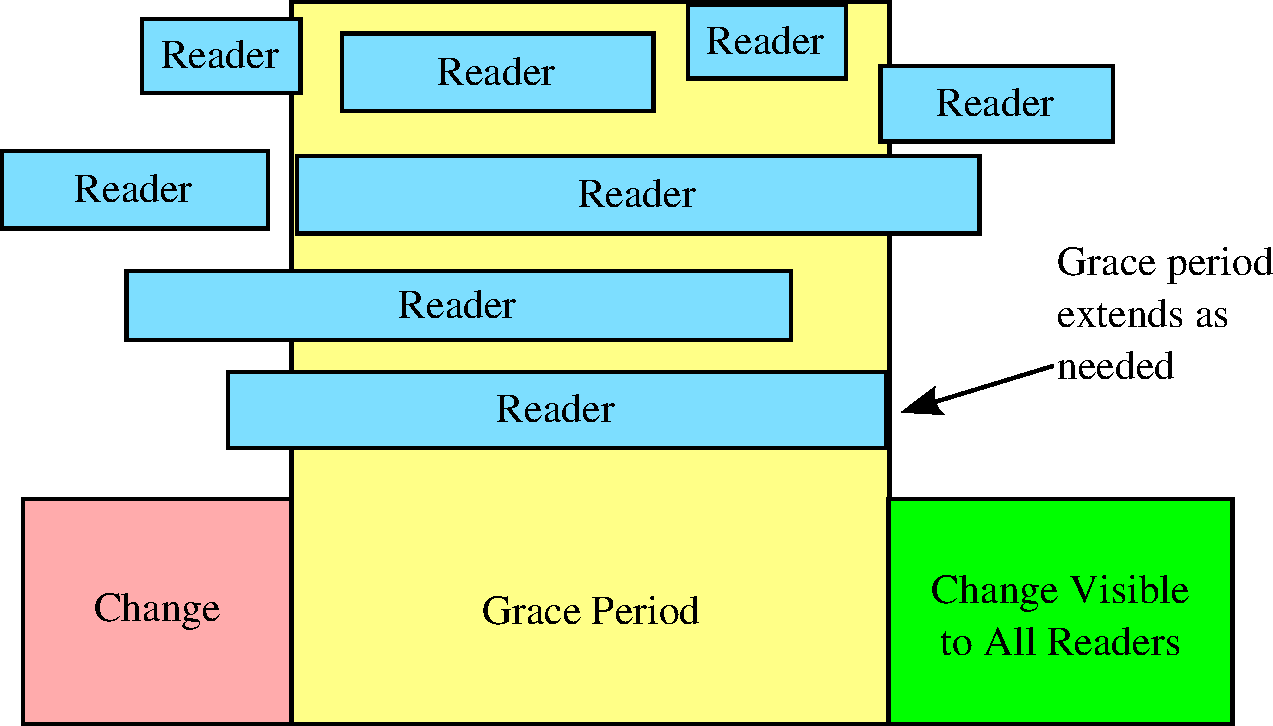
\includegraphics[scale=0.35]{rcu_concepts.pdf}
\caption{Поведение RCU}
\label{fig:rcu_concepts}
\end{figure}

\subsection{Программный интерфейс RCU} \label{sec:api_usage}
Программный интерфейс RCU достаточно невелик и состоит всего из пяти операций:
\co{rcu_read_lock()}, \co{rcu_read_unlock()}, \co{synchronize_rcu()},
\co{rcu_assign_pointer()}, and \co{rcu_dereference()}~\cite{McKenneyOSR08}.

Критическая секция RCU-читателя начинается с \co{rcu_read_lock()}
и заканчивается соответсвующим \co{rcu_read_unlock()}.
Вложенные критические секции чтения объединяются.
Внутри критической секции запрещается блокирование данного потока.
Данные, чтение которых осуществляется доступ внутри критической секции RCU,
будут доступны до её окончания.

Функция \co{synchronize_rcu()} соответсвует окончанию выполнения кода,
обновляющего значение объекта, тем самым сигнализируя о начале фазы освобождения.
Она блокирует поток-писатель до тех пор, пока все потоки-читатели
не выйдут из своих критических RCU-секций.
Отметим, что \co{synchronize_rcu()} не ожидает окончания
критических секций, вход в которые был осуществлен позже её вызова.

%\comment{Lihao: add example, e.g. http://paulmck.livejournal.com/39343.html}

\begin{figure}[tbp]
\centering
\footnotesize
\begin{verbatim}
               int x = 0;
               int y = 0;
               int r1, r2;

               void rcu_reader(void) {
                 rcu_read_lock();
                 r1 = x;
                 r2 = y;
                 rcu_read_unlock();
               }

               void rcu_updater(void) {
                 x = 1;
                 synchronize_rcu();
                 y = 1;
               }

               ...

               // after both rcu_reader()
               // and rcu_updater() return
               assert(r2 == 0 || r1 == 1);
\end{verbatim}
\caption{Verifying RCU Grace Periods}
\label{fig:verify_rcu_gp}
\end{figure}

Рассмотрим пример, приведенный на рисунке~\ref{fig:verify_rcu_gp}.
Если вход в критическую секцию чтения функции \co{rcu_reader()} выполнится до
вызова \co{synchronize_rcu()} в \co{rcu_updater()}, то выход из ней должен быть
совершен до возврата из \co{synchronize_rcu()}, чтобы значение переменной
\co{r2} было равно 0. Если же вход в неё произойдет после возврата из
\co{synchronize_rcu()}, то значение \co{r1} будет равным 1.

Наконец, для присвоения нового значения указателю, защищенному RCU,
потоки-писатели должны использовать \co{rcu_assign_pointer()},
которая возвращает новое значение.
RCU-читатели могут использовать \co{rcu_dereference()} для чтения
указателя, защищенного RCU, который впоследствии может быть безопасно разыменован.
%Note that this API does not actually dereference the pointer.
%Instead, it only fetches the pointer for later dereferencing.
Возвращаемое ею значение является корректным лишь внутри критической секции.
% Lihao: include this in PhD thesis and the technical report
Функции \co{rcu_assign_pointer()} и \co{rcu_dereference()} используются в паре
для того, чтобы убедиться, что если данный поток-читатель разыменовывает
защищенный указатель на только что вставленный объект, операция разыменования
вернет корректное значение, а не недоинициализированный мусор.

            % Background
\section{Реализация Tree RCU}\label{sec:tree_rcu}

Основное преимущество RCU заключается в том, что он позволяет
ожидать выхода весьма большого числа потоков-читателей из своих
критических секций без необходимости учета каждого из них:
в ядрах с non-preemptible реализацией многопоточности их число
ограничено количеством ядер процессора,
в ядрах с preemptible реализацией --- неограниченно вовсе.
Несмотря на то, что примитивы чтения RCU обладают замечательными
показателями производительности и масштабируемости,
примитивы записи должны оттягивать фазу освобождения до тех пор,
пока все потоки-читатели не выйдут из своих критических секций,
за счет блокирования или регистрации callback'а, который должен быть
вызван по истечении grace-периода.
Производительность и масштабируемость RCU определяются
эффективности механизмов обнаружения окончания \emph{grace}-периода.
Например, простейшая реализация RCU может требовать,
чтобы каждое ядро процессора использовало глобальную блокировку
для каждого grace-периода, но этот подход существенно снизит
производительность и масштабируемость.
Для реальных систем, имеющих тысячи процессоров и управляемых Linux,
данный подход неприменим. Этот факт послужил причиной создания Tree RCU.

\subsection{Обзор}
% Lihao: include this in PhD thesis; also look for 'preemptible RCU contents'
%There are several flavors of RCU, including RCU-sched, RCU-preempt,
%RCU Bot\-tom-Half, and Sleepable RCU (SRCU)~\cite{MckenneyRCUflavors}.
% Different flavors have different quiescent states, which are
% discussed in Section \ref{sec:quiescent_state}.
%
% Classic RCU has two implementations: Tiny RCU and Tree RCU. Tiny RCU
% is only for uni-processor systems; we therefore focus on Tree RCU in this paper.
% Tree RCU further has non-pre\-emptible and preemptible variants,
% configured by the kernel Kconfig option \co{CONFIG_PREEMPT}.
% There is no preemptible implementation of Tiny RCU: Instead,
% preemptible Tree RCU is used in single-CPU preemptible kernel builds.
%
% Tree RCU implements RCU-sched, RCU-bh, and RCU-preempt when \co{CONFIG_PREEMPT=y}.
% If \co{CONFIG_PREEMPT=n}, then RCU-preempt is mapped into RCU-sched.
% Tiny RCU requires \co{CONFIG_PREEMPT=n}, so it also maps
% RCU-preempt into RCU-sched.
%
Будем рассматривать <<стандартный>> программный интерфейс RCU
в комбинации с non-preemptible версией ядра Linux,
концентрируясь в основном на примитивах
\co{rcu_read_lock()}, \co{rcu_read_unlock()} и \co{synchronize_rcu()}.
%
%\comment{Lihao: it seems the Tree implementation of Classic RCU also
%implements other three flavors: RCU-sched, RCU-bh, and RCU-preempt;
%and Tiny RCU implements RCU-sched and RCU-bh. Am I right?
%Conceptually, what is the relationship between flavors Classic RCU and
%RCU-sched/RCU-bh? I shall discuss their relationship here otherwise
%readers may get confused when we discuss different flavors in the
%Tree RCU implementation in later sections.}
%\comment{Paul:
%	Yes, Tree RCU implements RCU-sched, RCU-bh, and RCU-preempt,
%	but only when \co{CONFIG_PREEMPT=y}.
%	If \co{CONFIG_PREEMPT=n}, then RCU-preempt is mapped into
%	RCU-sched.
%	Because Tiny RCU is requires \co{CONFIG_PREEMPT=n}, it behaves
%	the same as does Tree RCU when \co{CONFIG_PREEMPT=n},
%	implementing RCU-sched and RCU-bh, and mapping RCU-preempt into
%	RCU-sched.
%	For RCU-preempt, any location outside of an RCU read-side
%	critical section is a quiescent state.
%	For RCU-sched, context switch, idle, userspace,
%	\co{cond_resched_rcu_qs()}, and offline are all quiescent
%	states.
%	For RCU-bh, any location where bottom-half execution is enabled
%	is a quiescent state.
%	Use RCU-sched when you need updaters to wait on hardware interrupt
%	handlers (device drivers) or preempt-disable regions (tracing).
%	Use RCU-bh when networking denial-of-service attacks are a potential
%	issue.}
%
% In a non-pre\-empt\-ible kernel, Tiny and Tree RCU use the same
% \co{rcu_read_lock()} and \co{rcu_read_unlock()} implementation.
% Tiny RCU's \co{synchronize_rcu()} implementation is trivial,
% while preemptible and non-pre\-emptible Tree RCU largely share a rather
% elaborate implementation.
%
Основная идея заключается в том, что примитивы чтения RCU являются
частью ядра и поэтому в его non-preemptible конфигурациях не блокируются.
Поэтому каждый раз, когда ядро процессора простаивает в состоянии бездействия
или блокируется в процессе выполнения пользовательских программ,
все критические секции чтения RCU, запущенные ранее на этом ядре,
оказываются завершенными.
Поэтому каждое из этих состояний называется \emph{устойчивым состоянием}.
Каждый такой переход через устойчивое состояние сигнализирует об
окончании соответствующего grace-периода.
%\comment{Paul: Shouldn't the definition of quiescent state be before the
%first use?}
%\comment{Lihao: move here from the Read-Side Primitives subsection}
% \comment{Lihao: add an overview and high-level idea of how the implementation of Tree RCU works.}
Основная сложность заключается в том, чтобы определить момент,
когда все необходимые устойчивые состояния были пройлены для данного
grace-периода, сохранив при этом высокую производительность и масштабируемость.

Например, использование единой структуры данных для регистрации устойчивых
состояний каждого ядра приводит к неприемлемо частому использованию
блокировок на крупных системах, что в свою очередь приводит к снижению
производительности.
Для решения этой проблемы Tree RCU использует иерархическую организацию
структур данных, каждый узел которой предназначен для учета устойчивых
состояний отдельного ядра и предоставляет свою информацию более высоким уровням.
По достижении корня дерева grace-период заканчивается и
его информация распространяется по всем узлам-потомкам.
Вскоре после того, как узлы получают данную информацию,
происходит возврат из \co{synchronize_rcu()}.

В оставшейся части данного раздела мы рассмотрим реализацию Tree RCU
в non-preemptible конфигурации ядра Linux версии 4.3.6.
Вначале мы бегло опишем реализацию примитивов чтения и записи,
затем опишем иерархическую структуру данных, используемую для эффективного
учета устойчивых состояния, и, наконец, рассмотрим, как RCU использует
эту структуру данных для фиксации устойчивых состояний и grace-периодов
без учета отдельных потоков-читателей.

%\subsection{Read-Side Primitives} \label{sec:read_api_impl}
\subsection{Read/Write-Side Primitives} \label{sec:api_impl}
% Change in recent kernels.
В non-preemptible версии ядра любая область его исходного кода,
которая не использует добровольных блокировок, является неявной
критической секцией чтения RCU. В связи с этим, реализации
\co{rcu_read_lock()} и \co{rcu_read_unlock()} не должны выполнять
никакой работы. Действительно, в production сборках ядра
с выключенным режимом отладки, эта пара примитивов является
пустышками.

В общем случае, когда используется несколько вычислительных ядер процессора,
примитив записи \co{synchronize_rcu()} вызывает \co{wait_rcu_gp()},
которая является внутренней функцией, использующей механизм callback'ов
для отложенного вызова \co{wakeme_after_rcu()} по окончании некоторого grace-периода.
Как подсказывает название, данная функция повторно предназначена для повторного вызова
\co{wait_rcu_gp()}, которая на этот раз ничего не делает,
тем самым позволяя \co{synchronize_rcu()} вернуть управление в вызывающий поток.

%\comment{Lihao: comment out the following preemptible RCU contents if we need space.}
%In a preemptible kernel, \co{synchronize_rcu()} is implemented in
%\co{kernel/rcu/tree_plugin.h}. It first checks whether the variable
%\co{rcu_scheduler_active} is zero. If so, the system is so early in boot
%that there is only one non-preemptible task, again meaning that grace
%periods complete instantaneously, allowing an immediate return.
%Otherwise, if the grace period should be expedited,
%\co{synchronize_rcu_expedited()} is invoked.
%Otherwise, it passes \co{call_rcu()} to \co{wait_rcu_gp()}, which
%registers callback \co{wakeme_after_rcu()}, similar to
%the non-preemptible kernel discussed above.
%%\comment{Lihao: the source code comments state that \co{rcu_scheduler_active = 0}
%%allows RCU to optimize \co{synchronize_sched()} to a simple \co{barrier()}.
%%Where is the code that does this?}
%%\comment{Paul: The comment is incorrect.
%%The \co{synchronize_sched()} function instead checks the number of
%%online CPUs.
%%I have queued a patch with your
%%Reported-by changing the comment's \co{synchronize_sched()} to
%%\co{synchronize_rcu()}.}
%
%RCU's callback handling and grace period detection are explained in Sections
%\ref{sec:rcu_data} and \ref{sec:grace_period}, respectively.

% Lihao: understand how call_rcu_sched works and understand the differences from
% the Tiny RCU version which only calls the kernel function cond_resched()
%
% Lihao: In a preemptible kernel, the implementation of \co{synchronize_rcu()}
% http://lxr.free-electrons.com/source/kernel/rcu/tree_plugin.h#L539 and
% understand the differences between preemptible and non-preemptible versions

\subsection{Структуры данных Tree RCU} \label{sec:data_structure}

\begin{figure}[tbp]
\centering
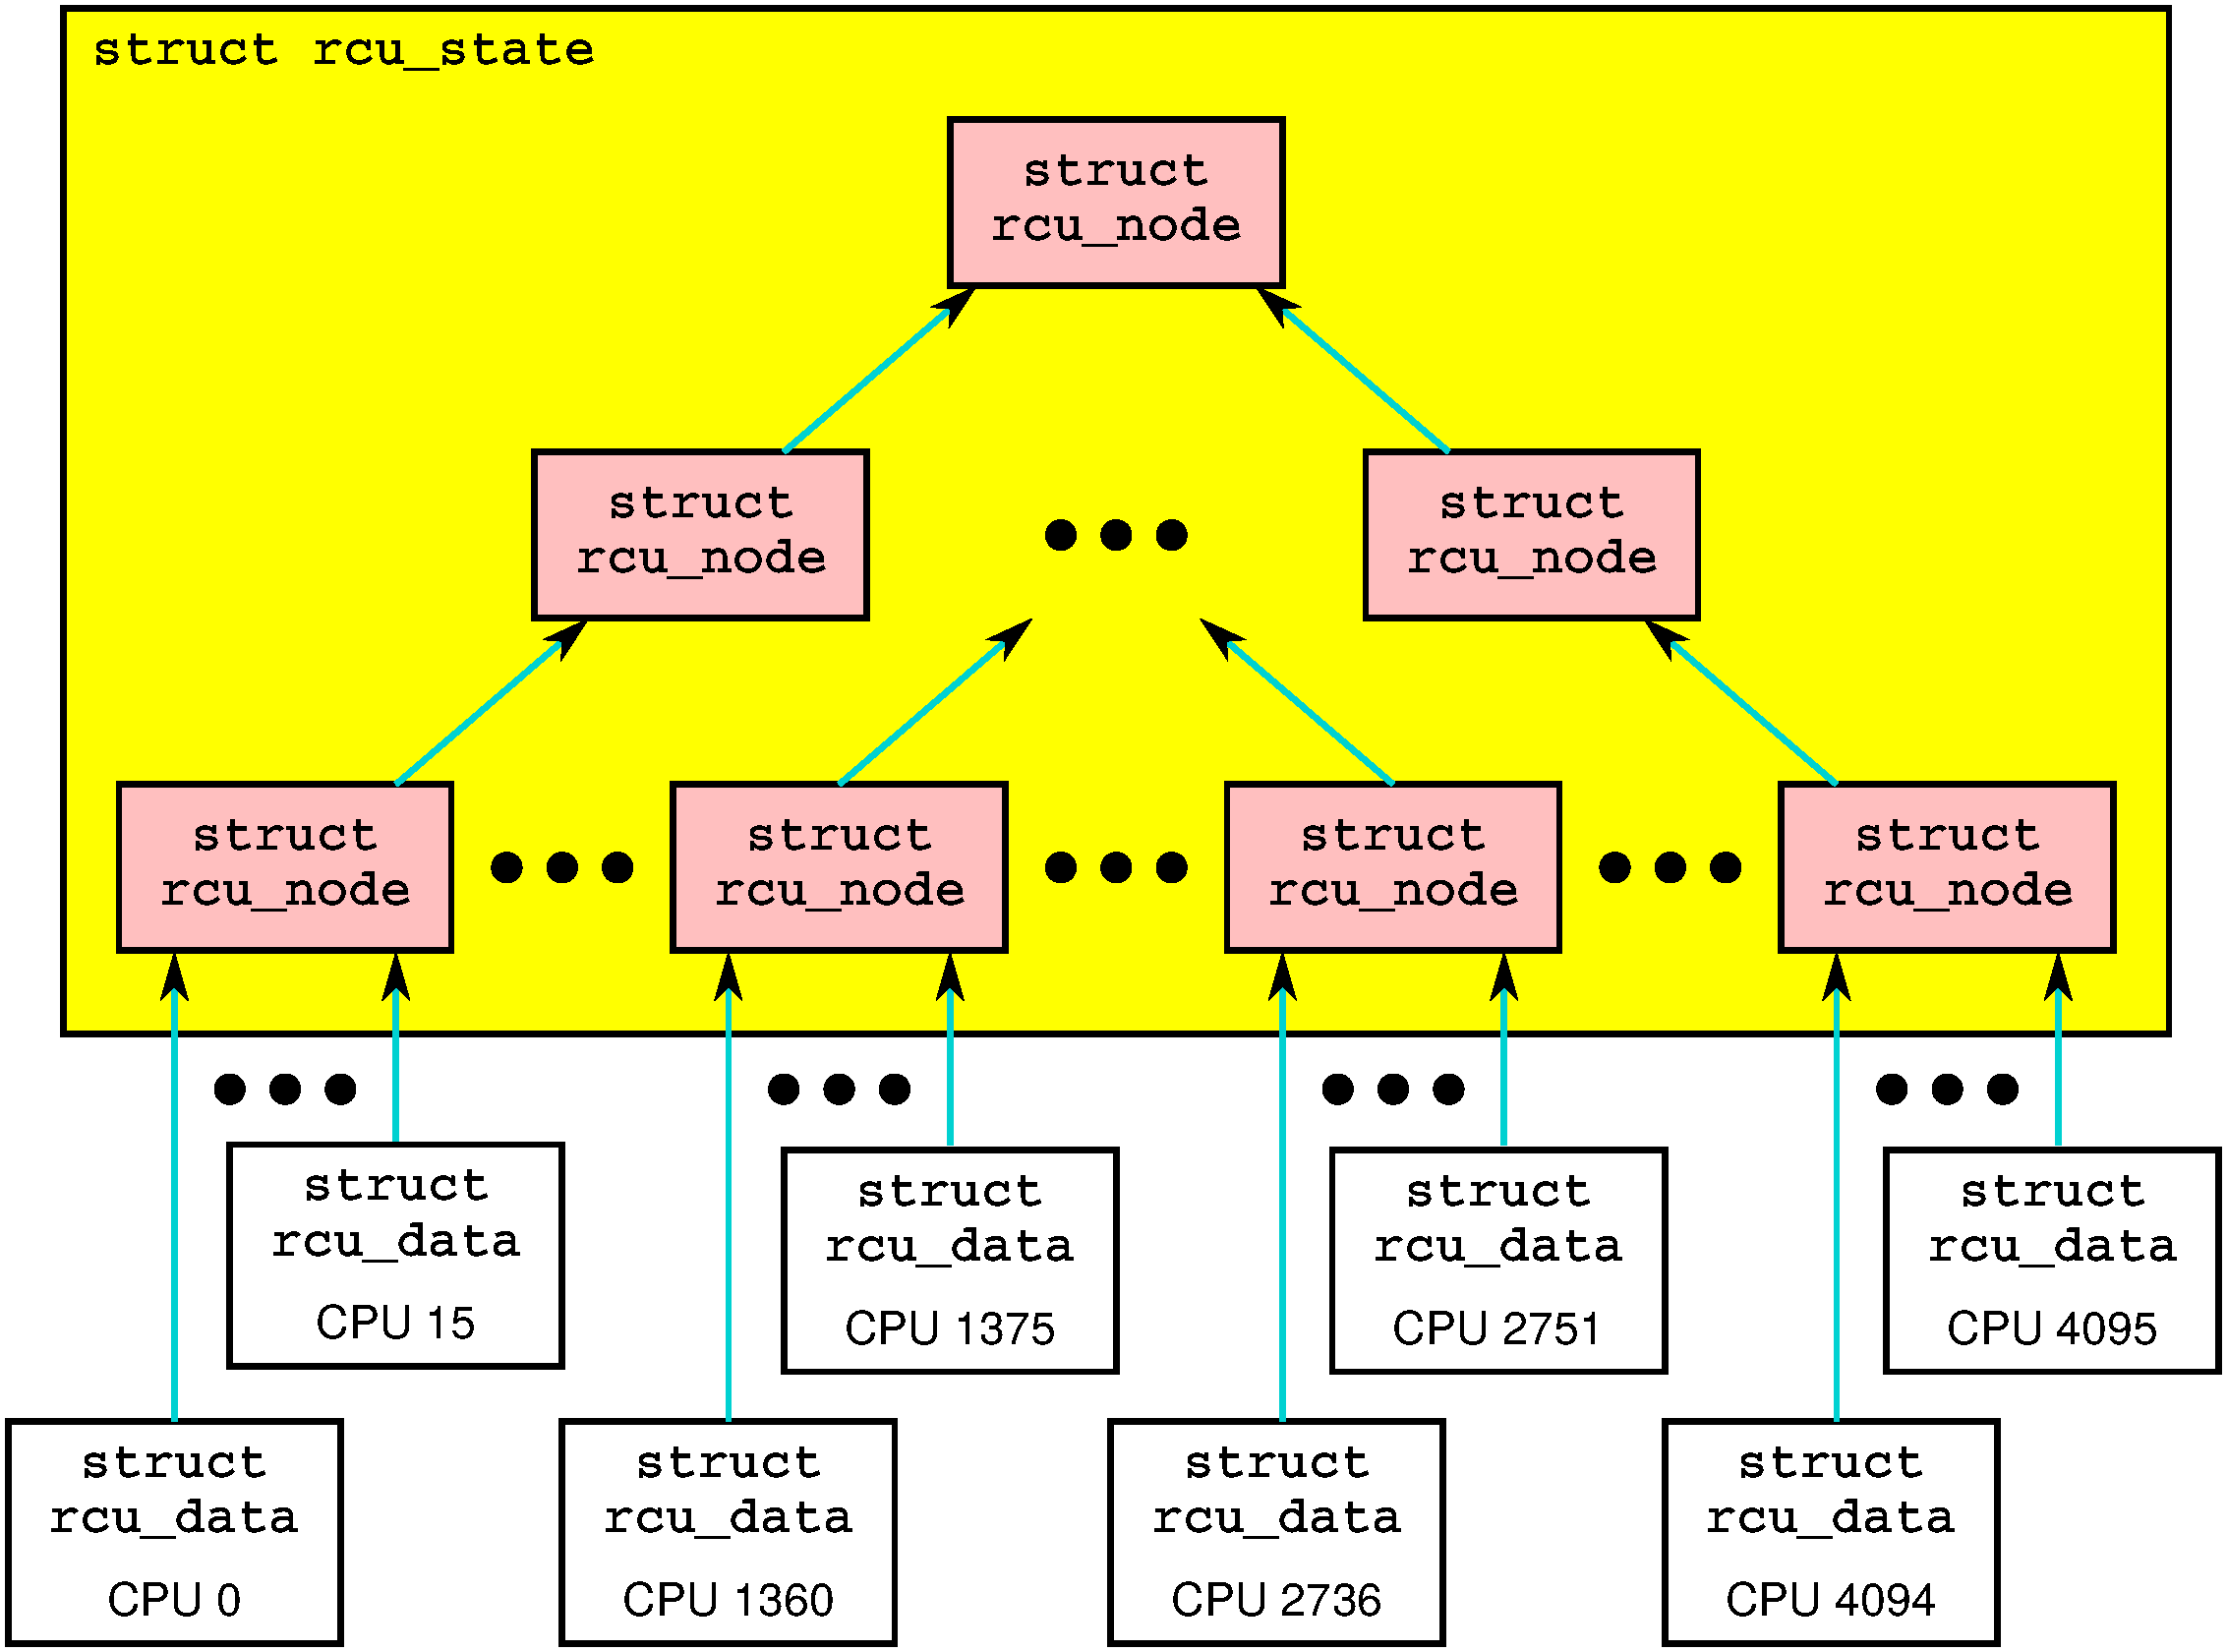
\includegraphics[scale=0.2]{tree_rcu_hierarchy.pdf}
\caption{Иерархия Tree RCU}
\label{fig:tree_rcu_hierarchy}
\end{figure}

Глобальное состояние RCU записывается в структуру \co{rcu_state},
представляющую собой дерево структур \co{rcu_node} с арностью, равной 64
(32 на 32-битных системах). Каждый терминальный узел данного дерева
может иметь ссылки на максимум 64 (32 на 32-битных системах) структуры
\co{rcu_data} каждая из которых соответствует отдельному ядру процессора,
как показано на рисунке~\ref{fig:tree_rcu_hierarchy}.
Каждая структура \co{rcu_data} ведет учет устойчивых состояний своего ядра,
а \co{rcu_node}-дерево используется сначала для распространения информации
об этих состояниях в направлении корня,
а затем --- для распространия информации о grace-периодах в направлении листьев.
Информация об устойчивых состояниях передается на родительский уровень
в тот момент времени, когда каждый узел-потомок каждого поддерева данного уровня
уже передал её в корень этого поддерева.
Эта схема передачи информации позволяет существенно сократить частоту использования
блокировок на верхних уровнях дерева.
Например, рассмотрим стандартное \co{rcu_node} дерево для системы с
4{,}096 вычислительными ядрами, имеющее 256 терминальных узлов,
4 внутренних узлов и один корневой узел. В течение данного grace-периода,
каждое ядро процессора сообщит информацию о своем устойчивом состоянии в
соответствующий терминальный узел, но при этом каждому терминальному узлу
будет соответствовать всего 16 соперничающих ядер.
Всего 256 ядер будут пытаться сообщить свои устойчивые состояния внутренним узлам,
при этом всего информация 64 ядер дойдет до каждого из четырех внутренних узов.
Наконец, информация всего четырех ядер может дойти до корневого узла,
что приводит к очень низкой частоте его блокирования.
Это позволяет использовать данную структуру на очень больших системах.
В частности, существующая реализация RCU ядра Linux поддерживает
четырехуровневые деревья, что позволяет использовать до
$64^4 = 16{,}777{,}216$ ядрами на 64-битных системах.\footnote{
  В настоящее время четырехуровневые деревья используются при нагрузочном тестировании,
  а трехуровневые находят свое применение на промышленных 4096-ядерных системах.}

\subsubsection{Структура \co{rcu_state}}

\begin{figure}[tbp]
\centering
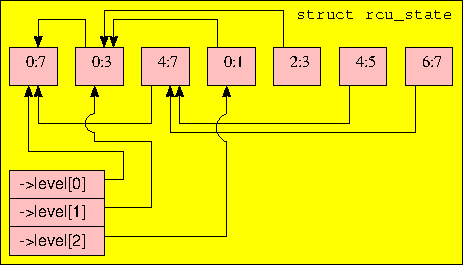
\includegraphics[scale=0.9]{rcu_node_array.pdf}
\caption{Представление дерева структур \co{rcu_node} в виде массива}
\label{fig:rcu_node_array}
\end{figure}

Каждая реализация RCU имеет свою собственную структуру \co{rcu_state}.
Структура \co{rcu_state} включает в себя массив структур \co{rcu_node},
логически организованных в виде дерева \co{struct rcu_node node[NUM_RCU_NODES]},
со структурами \co{rcu_data}, присоединенными к его терминальным узлам.
Таким образом, обход этого дерева в ширину сводится к линейному проходу по массиву.
Еще один массив структур \co{rcu_node}, \co{*level[NUM_RCU_LVLS]},
используется для указания на самый левый узел каждого уровня дерева,
как показано на рисунке~\ref{fig:rcu_node_array}.

Структура \co{rcu_state} использует поля \co{->gpnum} и \co{->completed}
типа \co{unsigned long} для учета grace-периодов.
Поле \co{->gpnum} используется для отслеживания начала последнего grace-периода,
в то время как \co{->completed} отслеживает окончание последнего grace-периода.
Если значения данных полей одинаковы, то RCU находится в состоянии по умолчанию.
Если же значение \co{gpnum} больше, чем \co{completed}, то RCU находится в состоянии
grace-периода. Все прочие комбинации являюется недопустимыми.

\subsubsection{Структура \co{rcu_node}}
\label{sec:rcu_node}
Дерево структур \co{rcu_node} регистрирует и распространяет
информацию об устойчивых состояниях от терминальных узлов к корневому,
а также распространяет информацию о grace-периодах в обратном направлении.
Структура \co{rcu_node} использует спин-блокировку \co{->lock} для защиты
своих полей. Поле \co{->parent} содержит указатель на струтуру-родителя,
при этом значение данного поля у корневого узла равно \co{NULL}.
Значение поля \co{->level} равно номеру уровня,
на котором находится данный узел в дереве,
считая уровень корневого узла нулевыми.
Поле \co{->grpmask} описывает номер бита данного узла в значении поля
\co{->qsmask} узла-родителя.
Поля \co{->grplo} и \co{->grphi} соответствуют наименьшему и наибольшему
порядковому номеру вычислительного ядра, учитываемого данной структурой.

Поле \co{->qsmask} указывает, какие из узлов-потомков еще не сообщили
о своих устойчивых состояниях на данный момент времени.
Как и в случае с \co{rcu_state}, структура \co{rcu_node} имеет поля
\co{->completed} и \co{->gpnum}, имеющие такие же значения, как и у родительской
структуры \co{rcu_state}, за исключением начала и конца каждого
grace-периода, когда данные значения копируются из корневого узла.
Значения этих полей могут быть равны друг другу, либо отличаться на единицу.

\subsubsection{Структура \co{rcu_data}} \label{sec:rcu_data}
Структурв \co{rcu_data} используется для учета устойчивых состояний и
вызова callback'ов связанного вычислительного ядра.
Поскольку доступ к данной структуре только осуществляется посредством
связанного вычислительного ядра, нет необходимости выполнять синхронизацию.
Как и в случае со структурой \co{rcu_state}, различные реализации RCU поддерживают
различные виды структур \co{rcu_data}.
Поле \co{->cpu} указывает на связанное вычислительное ядро,
\co{->rsp} --- на связанную структуру \co{rcu_state},
а \co{->mynode} ссылается на соответсвующую терминальную структуру \co{rcu_node}.
Значение поля \co{->grpmask} указывает на позицию структуры \co{rcu_data}
в битовом поле \co{->qsmask} связанной структуры \co{rcu_node}.

Структура \co{rcu_data} содержит поле \co{->qs_pending}, указывающее,
что RCU ожидает получения устойчивого состояния от связанного ядра,
и поле \co{->passed_quiesce}, указывающее на то, что данное ядро уже
прошло через устойчивое состояние.
Кроме этого, данная структура имеет поля \co{->gpnum} и \co{->completed},
значения которых могут отставать от соответсвующих им полей структур
\co{rcu_state} и \co{rcu_node} в режиме простоя ядер процессора.
С другой стороны, если ядра процессора являются заблокированными,
их значения могут оставать лишь на один grace-период от соответсвующих значений
полей структуры \co{rcu_node}.

Поля \co{->gpnum} и \co{->completed} структуры \co{rcu_state} содержат наиболее
актуальные значения и используются для обновления соответствующих полей родительских
структур \co{rcu_node}, что позволяет сравнивать значения данных полей со значениями
этих же полей структур \co{rcu_node} для фиксации факта начала очередного grace-периода.
Эта схема позволяет вычислительным ядрам обнаруживать границы grace-периодов
без использования блокировок.
Структруа \co{rcu_data} управляет RCU callback'ами с помощью
структуры данных, известной как четырехсегментный
список~\cite{LaiJiangshan2008NewClassicAlgorithm}.

\begin{figure}[tbp]
\centering
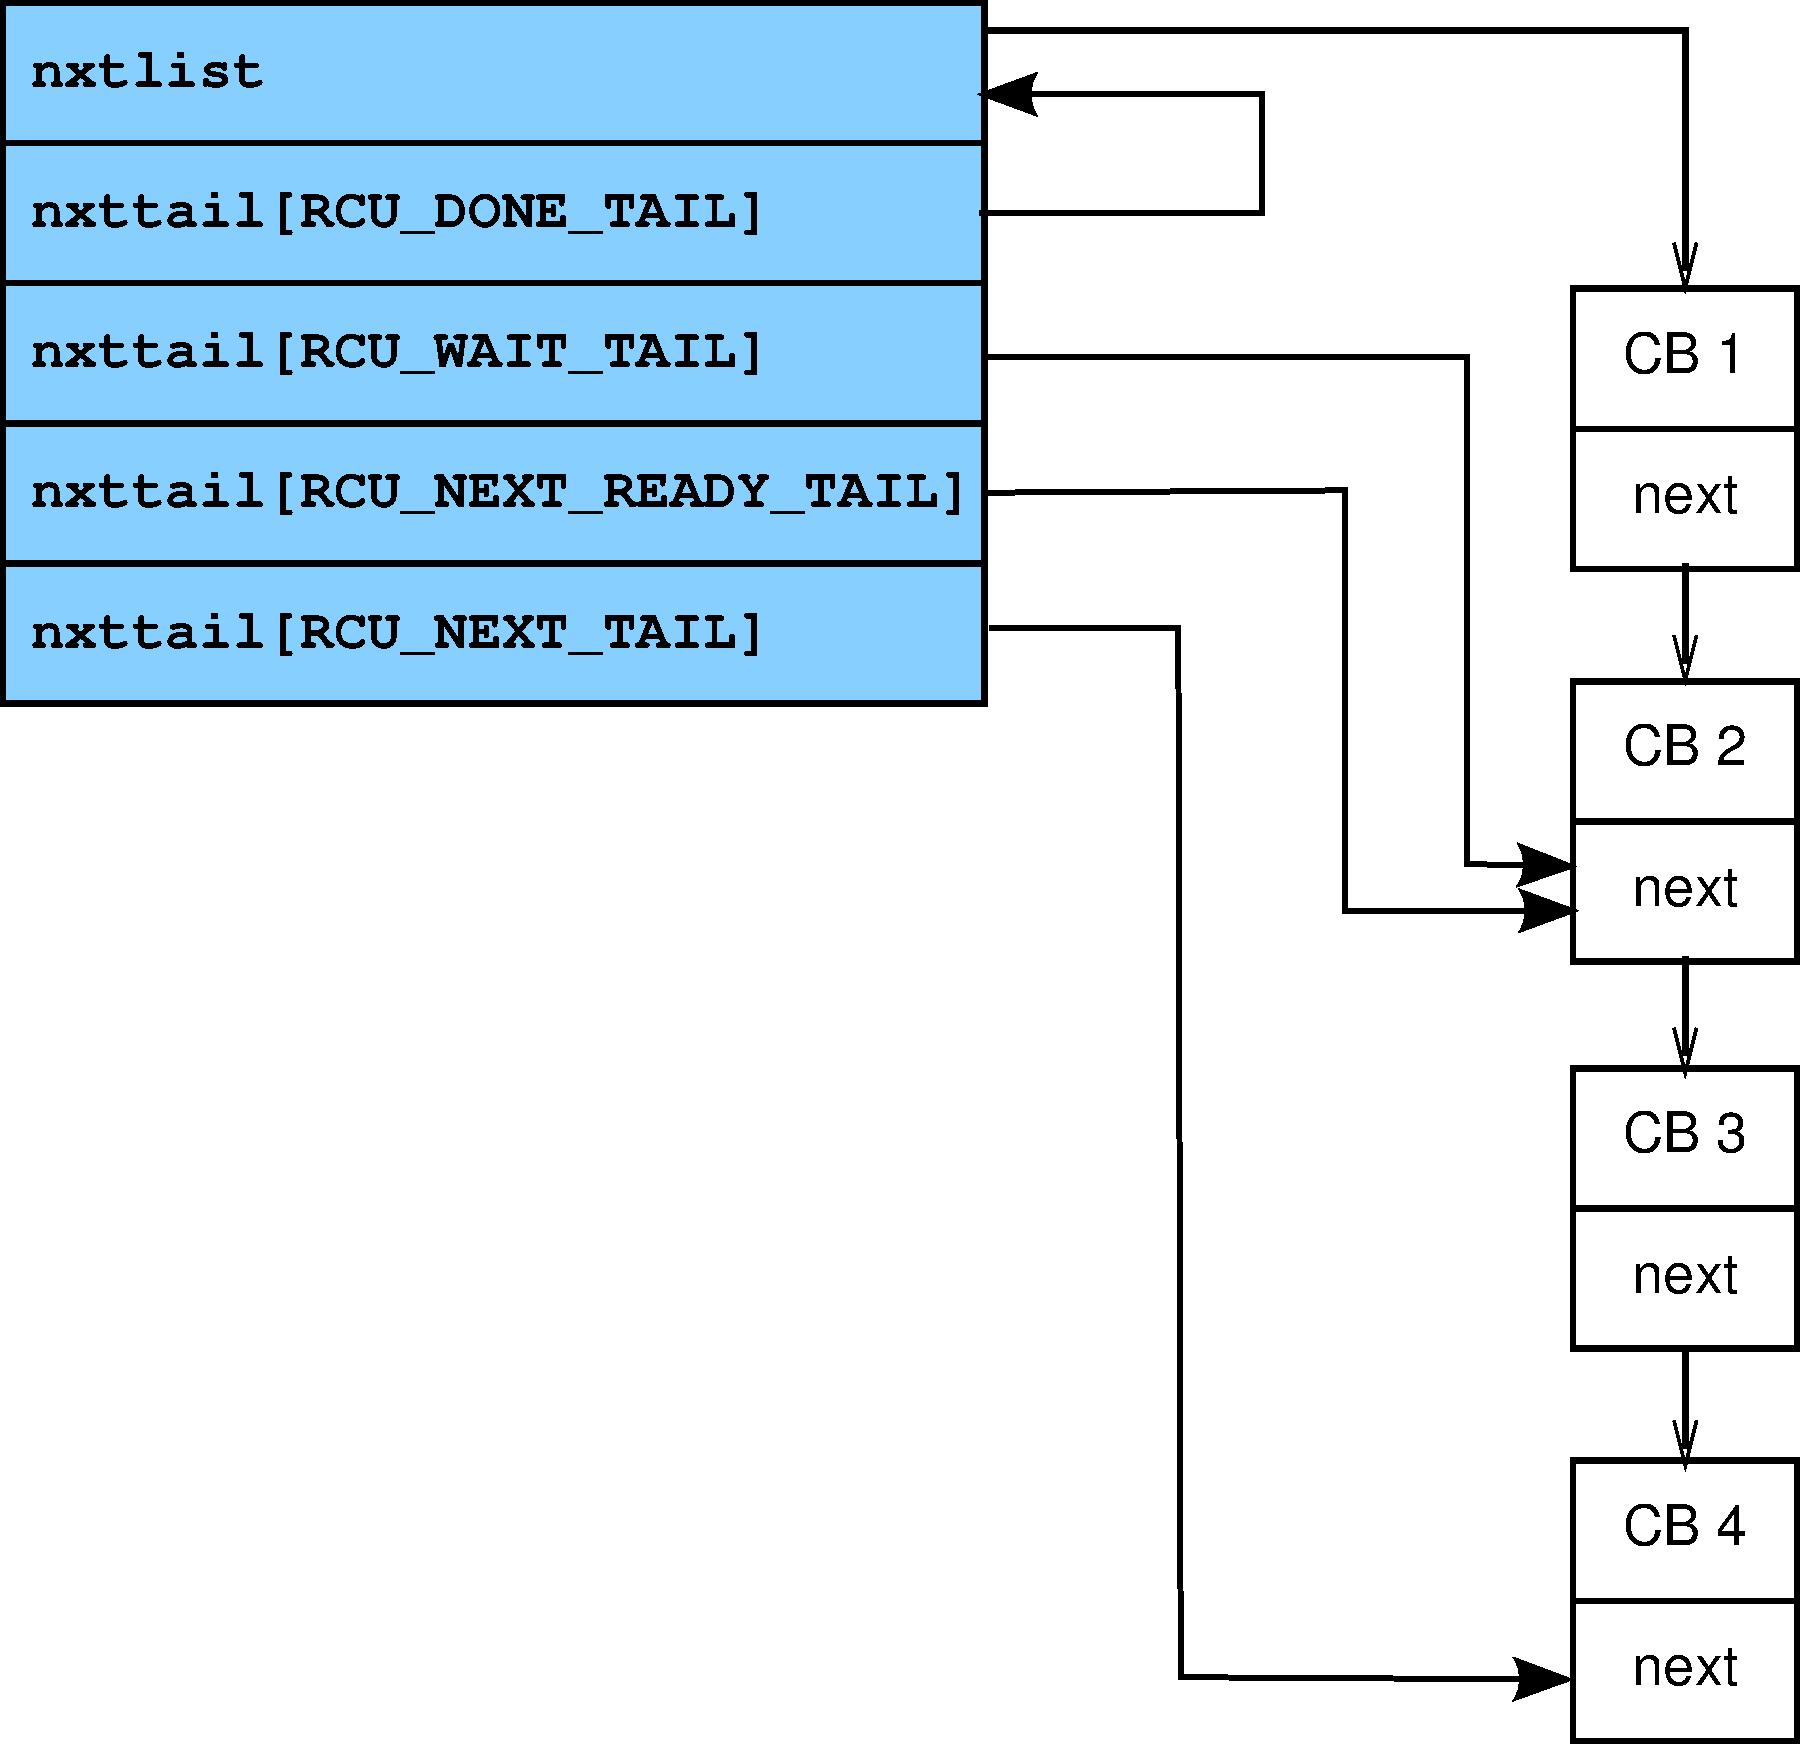
\includegraphics[scale=0.25]{rcu_data_callbacks.pdf}
\caption{Callback Queuing in \co{rcu_data}}
\label{fig:rcu_data_callbacks}
\end{figure}

%\comment{Lihao: since we don't model callbacks, only describe them briefly and add a reference
%to save space for the experiments section which is the main contribution of this paper. 
%Do the same for discussion of preemptible RCU.}
\subsubsection{RCU Callbacks}
The \co{rcu_data} structure manages RCU callbacks using a \co{->nxtlist}
pointer tracking the head of the list and an array of \co{->nxttail[]}
tail pointers that form a four-segment list of
callbacks~\cite{LaiJiangshan2008NewClassicAlgorithm}, with
each element of the \co{->nxttail[]} array referencing the tail of the
corresponding segment, as shown in Figure~\ref{fig:rcu_data_callbacks}.
The segment ending with \co{->nxttail[RCU_DONE_TAIL]} (the ``\co{RCU_DONE_TAIL}
segment'') contains callbacks
handled by a prior grace period that are therefore ready to be invoked.
The \co{RCU_WAIT_TAIL} and \co{RCU_NEXT_READY_TAIL} segments 
contain callbacks waiting for the
current and the next grace period, respectively.
Finally, the \co{RCU_NEXT_TAIL} segment contains
callbacks that are not yet associated with any grace period.
%
The \co{->qlen} field counts the total number of callbacks, and
the \co{->blimit} field specifies the maximum number of RCU callbacks
that may be invoked at a given time, thus limiting response-time
degradation due to long lists of callbacks.\footnote{
	Workloads requiring aggressive real-time guarantees should use
	callback offloading, which is outside of the scope of this paper.}

Back in Figure~\ref{fig:rcu_data_callbacks}, the
\co{->nxttail[RCU_DONE_TAIL]} array element references \co{->nxtlist}, 
which means none of the callbacks are ready to invoke.
The \co{->nxttail[RCU_WAIT_TAIL]} element references callback 2's \co{->next}
pointer, meaning that callbacks CB~1 and CB~2 are waiting for the current
grace period.
The \co{->nxttail[RCU_NEXT_READY_TAIL]} element references that same \co{->next}
pointer, meaning that no callbacks are waiting for the next grace period. 
Finally, the callbacks between the \co{->nxttail[RCU_NEXT_READY_TAIL]} and
\co{->nxttail[RCU_NEXT_TAIL]} elements (CB~3 and CB~4)
are not yet assigned to a specific grace period.
The \co{->nxttail[RCU_NEXT_TAIL]} element always references either
the last callback or, when the entire list is empty, \co{->nxtlist}.

Cache locality is promoted by invoking callbacks on the CPU that registered
them.
For example, RCU's update-side primitive 
\co{synchronize_rcu()} appends callback \co{wakeme_after_rcu()} to the end
of the \co{->nxttail[RCU_NEXT_TAIL]} list in the current CPU 
(Section \ref{sec:update_api_impl}). 
They are advanced one segment towards the head of the list (via \co{rcu_advance_cbs()}) 
when the CPU detects the current grace period has ended, which is indicated 
by the \co{->completed} field of the CPU's \co{rcu_data} structure being one
smaller than its counterpart in the corresponding leaf \co{rcu_node} structure.
The CPU also periodically merges the \co{RCU_NEXT_TAIL} segment into the
\co{RCU_NEXT_READY_TAIL} segment by calling \co{rcu_accelerate_cbs()}.
In a few special cases, the CPU merges the \co{RCU_NEXT_TAIL} segment
into the \co{RCU_WAIT_TAIL} segment, bypassing the \co{RCU_NEXT_TAIL}
segment.
This optimization applies when the CPU is starting a new grace period.
It does \emph{not} apply when a CPU notices a new grace period
because that grace period might well have started before
the callbacks were added to the \co{RCU_NEXT_TAIL} segment.
%\comment{Lihao: why can't we invoke *all* callbacks when starting a new 
%grace period? Isn't it true that all pre-existing read-side critical
%sections, i.e.~those start before callbacks are registered in \co{->nxttail} 
%(in particular \co{wakeme_after_rcu} in \co{->nxttail[RCU_NEXT_TAIL]}), 
%have finished?}
%\comment{Paul: In theory, we could, but in practice doing this would
%have several disadvantages:
%(1) All callbacks would be invoked by the grace-period kthread, and
%large systems could generate more callbacks than a single CPU could
%keep up with, which would delay subsequent grace periods and possibly
%even run the system out of memory.
%(2) Running all the callbacks at once could degrade real-time response.
%(3) Running callbacks on a different CPU than the one that registered
%them would decrease locality, increasing cache-miss rates, thus degrading
%performance.
%(4) This would require that atomic instructions be used when registering
%callbacks (as they are for no-CBs CPUs), further degrading performance.
%In addition, we could only invoke callbacks in the \co{RCU_NEXT_TAIL}
%segment, because callbacks in the later segments
%(\co{RCU_NEXT_READY_TAIL}, \co{RCU_WAIT_TAIL}, and
%\co{RCU_DONE_TAIL} might well have been queued \emph{after} the
%recently-completed grace period started.}
%
This is a deliberate design choice: It is more important for the CPUs
to operate independently (thus avoiding contention and synchronization
overhead) than it is to decrease grace-period latencies.
In those rare occasions where low grace-period latency is important,
the \co{synchronize_rcu_expedited()} should be used.
This function has the same semantics as does \co{synchronize_rcu()},
but trades off efficiency optimizations in favor of reduced latency.
% Lihao: this is where the callback of RCU's update API register? 
% Paul: Yes, call_rcu() appends the callback to the end of the current
% CPU's RCU_NEXT_TAIL list.  Ignoring callback offloading for the moment.
% Lihao: we don't model QS forcing and offline CPUs
% Paul: Nor are you modeling callback offloading.  Which is fine, just calling
% it out.  ;-)

Each RCU callbacks is an \co{rcu_head} structure which has a
\co{->next} field that points to the next callback on the list and
a \co{->func} field that references the function to be invoked at the
end of an upcoming grace period.




\subsection{Обнаружение устойчивых состояний} \label{sec:quiescent_state}
Механизм RCU должен ожидать до тех пор,
пока все потоки не выйдут из своих критических секций чтения перед тем,
как можно будет завершить grace-период.
Производительность и масштабируемость RCU
основывается на его способности быстро обнаруживать
устойчивые состояния вычислительных ядер и определять
момент, когда их набралось достаточно, чтобы завершить
grace-период.
Если каждое ядро (или, в случае preemptible-RCU, каждый поток)
прошел через устойчивое состояние, то можно считать,
что grace-период закончился.

В случае использования non-preemptible RCU-sched вида RCU,
устойчивыми состояниями считаются следующие состояния вычислительных ядер:
выполнение инструкций пользовательского пространства,
переключение контекста, режим ожидания и offline-режим.
RCU-sched отслеживает лишь потоки и векторы прерываний,
которые выполняются в данный момент,
поскольку заблокированные и прерванные потоки всегда находятся в
устойчивых состояниях.
Таким образом, RCU-sched достаточно отслеживать состояния вычислительных ядер.

\subsubsection{Таймер прерываний} \label{sec:timer_interrupt}
Функция \co{rcu_check_callbacks()} вызывается из обработчика таймера прерываний,
позволяющего RCU периодически проверять, находится ли данное вычислительное
ядро в пользовательском режиме или в одном из устойчивых состояний.
Если ядро находится в одном из этих состояний,
\co{rcu_check_callbacks()} вызывает \co{rcu_sched_qs()},
который изменяет значение поля \co{rcu_sched_data.passed_quiesce} для
каждого ядра.
Функция \co{rcu_check_callbacks()} вызывает \co{rcu_pending()}
для того, чтобы проверить, является ли последнее событие или данное условие
признаком внимания к данному ядру со стороны RCU.
Если да, то \co{rcu_check_callbacks()} вызывает функцию \co{raise_softirq()},
которая приводит к тому, что \co{rcu_process_callbacks()} будет вызвана,
как только ядро достигнет безопасного состояния
(грубо говоря, когда на ядре будут включены прерывания,
preemption и bottom halves).
Эта функция подробно рассматривается в разделе \ref{sec:grace_period}.

\subsubsection{Управление переключениями контекста} \label{sec:context_switch}
Устойчивые состояния, связанные с переключениями контекста,
учитываются путем вызова функции \co{rcu_note_context_switch()} из
\co{__schedule()}
(и, для поддержки виртуализации,
из \co{rcu_virt_note_context_switch()}).
Функция \co{rcu_note_context_switch()} вызывает \co{rcu_sched_qs()}
для оповещения RCU о переключении контекста, которое является устойчивым
состоянием вычислительного ядро.

\subsection{Grace Period Detection} \label{sec:grace_period}
Once each CPU has passed through a quiescent state, a grace period for RCU
has completed. 
As discussed in Section \ref{sec:data_structure}, Tree-RCU uses a hierarchy 
of \co{rcu_node} structures to manage quiescent state and grace period
information.
Quiescent-state information is passed up the 
tree from the leaf per-CPU \co{rcu_data} structures.
Grace-period information is passed down from the root.
%
%The dyntick-idle mechanisms used for idle CPUs and \co{nohz_full} userspace
%execution are out of scope for this research, as are RCU CPU stall warnings. The focus is instead 
We focus on grace-period detection for busy CPUs, as illustrated
in Figure~\ref{fig:grace_period_state_diagram}.

\begin{figure}[tb]
\centering
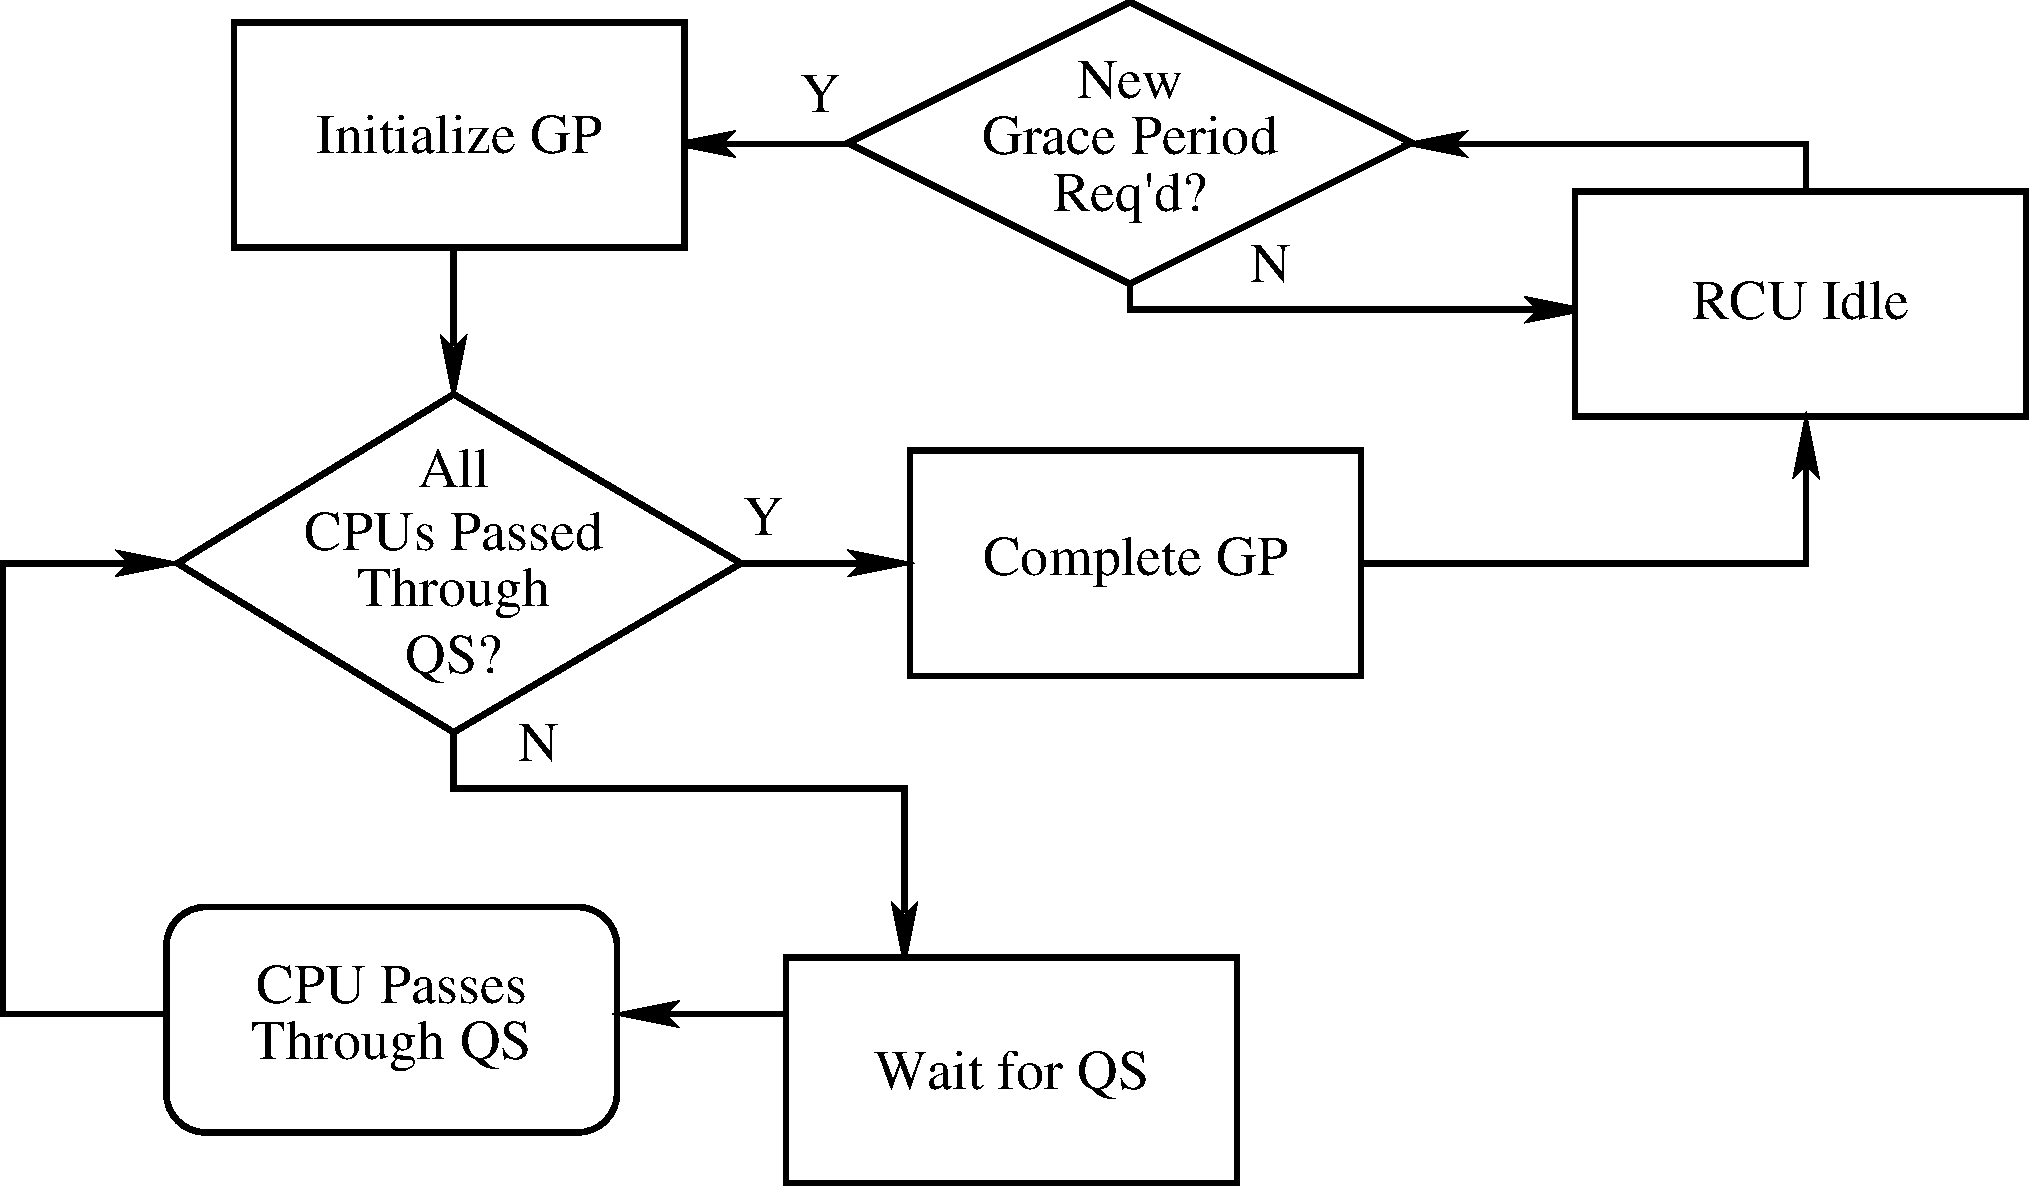
\includegraphics[scale=0.25]{grace_period_state_diagram.pdf}
\caption{Grace-Period Detection State Diagram}
\label{fig:grace_period_state_diagram}
\end{figure}

\subsubsection{Softirq Handler for RCU} \label{sec:rcu_softirq}
RCU's busy-CPU grace period detection relies on the
\co{RCU_SOFTIRQ} handler function \co{rcu_process_callbacks()},
which is scheduled from the scheduling-clock interrupt.
This function first calls
\co{rcu_check_quiescent_state()} to report recent quiescent states
on the current CPU.
Then \co{rcu_process_callbacks()} starts a new grace period if needed,
and finally calls \co{invoke_rcu_callbacks()} to invoke any callbacks
whose grace period has already elapsed.

Function \co{rcu_check_quiescent_state()} first invokes \co{note_gp_changes()} 
to update the CPU-local \co{rcu_data} structure to record the end of 
previous grace periods and the beginning of new grace periods.
%, which are detected via differences in the \co{->completed} and
%\co{->gpnum} fields, respectively.
Any new values for these fields are copied from the leaf \co{rcu_node}
structure to the \co{rcu_data} structure.
If an old grace period has ended, \co{rcu_advance_cbs()} is invoked to
advance all callbacks, otherwise, \co{rcu_accelerate_cbs()} is invoked
to assign a grace period to any recently arrived callbacks.
If a new grace period has started, \co{->passed_quiesce} is set to zero,
and if in addition RCU is waiting for a quiescent state from this CPU,
\co{->qs_pending} is set to one, so that a new quiescent state will
be detected for the new grace period.
%
% Lihao: this is one of the two places where qs_pending gets updated in Tree RCU
% \comment{(Lihao: does it mean even this softirq is invoked because of a quiescent state of this CPU
%   (\co{rdp->passed_quiesce} is set to 1 in \co{rcu_check_callbacks} so \co{rcu_pending} 
%   return 1), if for some reason gpnum in \co{rcu_data} of this CPU is one lag behind its parent 
%   counterpart, this CPU needs to wait for its next quiescent to commit? 
%   \url{http://lxr.free-electrons.com/source/kernel/rcu/tree.c#L1747}
% )}
% Paul: Yes.  I did look into immediately detecting quiescent states for
% RCU-preempt, but it didn't seem worth the coding contortions required.

Next,
\co{rcu_check_quiescent_state()} checks whether \co{->qs_pending} indicates
that RCU needs a quiescent state from this CPU.
If so, it checks whether \co{->passed_quiesce} indicates that this
CPU has in fact passed through a quiescent state.
If so, it invokes \co{rcu_report_qs_rdp()} to report that quiescent
state up the %\co{rcu_data} and \co{rcu_node} 
combining tree.

The \co{rcu_report_qs_rdp()} function first verifies that the CPU has
in fact detected a legitimate quiescent state for the current grace period,
and under the protection of the leaf \co{rcu_node} structure's \co{->lock}.
If not, it resets quiescent-state detection and returns, thus ignoring
any redundant quiescent states belonging to some earlier grace period.
Otherwise, if the \co{->qsmask} field indicates that RCU needs to report a 
quiescent state from this CPU, \co{rcu_accelerate_cbs()} is invoked to assign 
a grace-period number to any new callbacks, and then \co{rcu_report_qs_rnp()} 
is invoked to report the quiescent state to the \co{rcu_node} combining tree.

% \comment{(Lihao: did we just check this in \co{rcu_check_quiescent_state()}? 
%   \url{http://lxr.free-electrons.com/source/kernel/rcu/tree.c#L2394}
% )}
% \comment{(Lihao: but did we just update \co{rdp->gpnum = rnp->gpnum} in \co{note_gp_changes()}...?
%   are they just double-checks or something may happen in between which I miss?
% )}
% Paul:  The code could probably be simplified.  The first step is to
% add assertions to verify the suspicions, and if the assertions don't
% trigger over a period of a year or so, simplify the code.  Sometimes
% the assertions have triggered, hence the caution.  ;-)
%
% \comment{(Lihao: what are \co{rcu_qs_ctr} and \co{rcu_qs_ctr_snap} used for? 
%  \url{http://lxr.free-electrons.com/source/kernel/rcu/tree.c#L2341}
% )}
% Paul: These are used by cond_resched_rcu_qs(), which records a quiescent
% state for all flavors of RCU.
%
%
% \comment{(Lihao: can we use \co{rdp->qs_pending} in the following line of code since 
%  it's also get updated in \co{note_gp_changes()}, right? 
%  \url{http://lxr.free-electrons.com/source/kernel/rcu/tree.c#L2357}
%)}
%
% \comment{(Lihao: comments in \url{http://lxr.free-electrons.com/source/kernel/rcu/tree.c#L2272}
%   say if this CPU is the last one to pass through a quiescent state in the current grace period, 
%   \co{rcu_report_qs_rsp()} is invoked to do the clean up and let \co{rcu_start_gp()} 
%   start a new grace period if one is needed.~But where is \co{rcu_start_gp()} called in 
%   \co{rcu_report_qs_rsp()}?
% )}
% Paul: This is done indirectly by waking up the RCU grace-period kthread.

The \co{rcu_report_qs_rnp()} function traverses up the \co{rcu_node} tree,
at each level holding the \co{rcu_node} structure's \co{->lock}.
At any level, if the child structure's \co{->qsmask} bit is already clear,
or if the \co{->gpnum} changes, traversal stops.
Otherwise, the child structure's bit is cleared from \co{->qsmask},
after which, if \co{->qsmask} is non-zero, %or if any tasks are queued on the
%\co{->blkd_tasks} list (which applies only to RCU-preempt), 
traversal stops. Otherwise, traversal proceeds on to the parent \co{rcu_node} structure.
%If there is no parent (that is, the previous \co{rcu_node} structure was the root), 
%the current grace period has completed. In that case, traversal stops and 
Once the root is reached, traversal stops and \co{rcu_report_qs_rsp()} is
invoked to awaken the grace-period kthread (kernel thread).
The grace-period kthread will then clean up after the now-ended grace
period, and, if needed, start a new one.

\subsubsection{Grace-Period Kernel Thread} \label{sec:rcu_gp_kthread}
The RCU grace-period kthread invokes \co{rcu_gp_kthread()}, which
contains an infinite loop that initializes, waits for, and cleans up after
each grace period. 

% rcu_gp_init()
When no grace period is required, the grace-period kthread
sets its \co{rcu_state} structure's \co{->flags} field to
\co{RCU_GP_WAIT_GPS}, and then
waits within an inner infinite loop for that structure's
\co{->gp_state} field to be set.
Once set, \co{rcu_gp_kthread()} invokes \co{rcu_gp_init()} to initialize
a new grace period, which
rechecks the \co{->gp_state} field under
the root \co{rcu_node} structure's \co{->lock}.
If the field is no longer set, \co{rcu_gp_init()} returns zero.
Otherwise, it
increments \co{rsp->gpnum} by 1 to record a new grace period number.
%
Finally, it performs a breadth-first traversal of the \co{rcu_node}
structures in the combining tree.
For each \co{rcu_node} structure \co{rnp},
% drop preemptible RCU contents
%we invoke \co{rcu_preempt_check_blocked_tasks()}, which responds to
%a non-empty list of blocked tasks by setting \co{rnp->gp_tasks} to
%\co{rnp->blkd_tasks.next}, so that those tasks block the new grace period.
%
we set the \co{rnp->qsmask} to indicate which children
must report quiescent states for the new grace period (Section 
\ref{sec:rcu_node}), and set \co{rnp->gpnum} and \co{rnp->completed}
to their \co{rcu_state} counterparts. 
%
If the \co{rcu_node} structure \co{rnp} is the parent of the current CPU's \co{rcu_data}, 
we invoke \co{__note_gp_changes()} to set up the CPU-local \co{rcu_data} state. 
Other CPUs will invoke \co{__note_gp_changes()} after their next
scheduling-clock interrupt. %(Section~\ref{sec:timer_interrupt}).
 
%Note that other CPUs will access only the leaves of the hierarchy, thus seeing that 
%no grace period is in progress, at least until the corresponding leaf node has been 
%initialized. In addition, we have included CPU-hotplug operations since v4.1.

% Lihao: include this in PhD thesis; also look for 'preemptible RCU contents'
% rcu_gp_fqs()
%During a grace period, the grace-period kthread periodically
%calls \co{force_qs_rnp()} to detect idle and offline CPUs. 
%For each such CPU, \co{force_qs_rnp()} invokes \co{rcu_report_qs_rnp()}
%to report a quiescent state on its behalf, thus avoiding the degraded
%energy efficiency that would be incurred should RCU awaken idle CPUs.
%CPUs that fail to report quiescent states will be sent an
%inter-processor interrupt (IPI), and if that fails, warning messages
%will be emitted.

% rcu_gp_cleanup()
To clean up after a grace period, \co{rcu_gp_kthread()} 
calls \co{rcu_gp_cleanup()} after setting the \co{rcu_state} field \co{rsp->gp_state} 
to \co{RCU_GP_CLEANUP}. After the function returns, \co{rsp->gp_state} is set to 
\co{RCU_GP_CLEANED} to record the end of the old grace period.
%
Function \co{rcu_gp_cleanup()} performs a breadth-first traversal of
\co{rcu_node} combining-tree.
It first sets each \co{rcu_node} structure's \co{->completed} field
to the \co{rcu_state} structure's \co{->gpnum} field.
It then updates the current CPU's CPU-local \co{rcu_data} structure by
calling \co{__note_gp_changes()}. 
For other CPUs, the update will take place when they handle the scheduling-clock
interrupts, in a fashion similar to \co{rcu_gp_init()}. 
After the traversal, it marks the completion of the grace period by setting the
\co{rcu_state} structure's \co{->completed}
field to that structure's \co{->gpnum} field, and invokes
\co{rcu_advance_cbs()} to advance callbacks. 
%
Finally, if another grace period is needed,
we set \co{rsp->gp_flags} to \co{RCU_GP_FLAG_INIT}. 
Then in the next iteration of the outer loop, the grace-period kthread
will initialize a new grace period as discussed above.

% Lihao: understand how nodes in the tree sync with information for each grace period

% Lihao: Tree RCU starts a new grace by calling rcu_gp_kthread_wake() that wakes up 
% the rcu_gp_kthread() kernel thread which does the clean up and invokes rcu_gp_init() 
% to start a new grace period

% Lihao: other places that may start a new grace period 
% 1. rcu_check_quiescent_state() calls note_gp_changes() that checks 
% rcu_accelerate_cbs() or rcu_advance_cbs()
% 2. rcu_report_qs_rdp() by checking rcu_accelerate_cbs()
% 3. __rcu_process_callbacks() by checking cpu_needs_another_gp and rcu_start_gp() 
% which in turn calls rcu_advance_cbs() and rcu_start_gp_advanced
% 4. __call_rcu_core by checking rcu_start_gp() 
% 5. force_quiescent_state()


\section{Verification Scenario}
% \comment{Lihao: alternative titles: A Running Example? Putting Things Together?}

We use the example in Figure~\ref{fig:verify_rcu_gp} to demonstrate how the
different components of Tree RCU work together to guarantee that all
pre-existing read-side critical sections finish before RCU allows a grace
period to end.  This example will drive the verification, which will check
for violations of the assertion at this end of the code.

We focus on the implementation of the non-preemptible RCU-sched flavor.  We
further assume there are only two CPUs, and that CPU~0 executes function
\co{rcu_reader()} and CPU~1 executes \co{rcu_updater()}.  When the system
boots, the Linux kernel calls \co{rcu_init()} to initialize RCU, which
includes constructing the combining tree of \co{rcu_node} and \co{rcu_data}
structures via \co{rcu_init_geometry()} and initializing the fields of the
nodes in the tree for each RCU flavor via \co{rcu_init_one()}.  In our
example it will be a one-level tree that has one \co{rcu_node} structure as
root and two children that are \co{rcu_data} structures for each CPU. 
Function \co{rcu_spawn_gp_kthread()} is also called to initialize and spawn
the RCU grace-period kthread for each RCU flavor.

Referring again to Figure~\ref{fig:verify_rcu_gp},
suppose that \co{rcu_reader()} begins
execution on CPU~0 while \co{rcu_updater()} concurrently sets \co{x} to 1
and then invokes \co{synchronize_rcu()} on CPU~1.
As discussed in Section \ref{sec:api_impl}, \co{synchronize_rcu()}
invokes \co{wait_rcu_gp()}, which in turn registers an RCU callback
that will invoke \co{wakeme_after_rcu()} some time after \co{rcu_reader()}
exits its critical section.

However, this critical-section exit has no immediate effect.
Instead, a later context switch will invoke
\co{rcu_note_context_switch()}, which in turn invokes
\co{rcu_sched_qs()}, recording the quiescent state in the
CPU's \co{rcu_sched_data} structure's \co{->passed_quiesce} field.
Later, a scheduling-clock interrupt will invoke
\co{rcu_check_callbacks()}, which calls \co{rcu_pending()} and 
notes that the \co{->passed_quiesce} field is set.
This will cause \co{rcu_pending()} to return \co{true}, which
in turn causes \co{rcu_check_callbacks()} to invoke
\co{rcu_process_callbacks()}.
In its turn, \co{rcu_process_callbacks()} will invoke
\co{raise_softirq(RCU_SOFTIRQ)}, which,
once the CPU has interrupts, preemption, and
bottom halves enabled, %(Section \ref{sec:timer_interrupt}),
calls \co{rcu_process_callbacks()}.

As discussed in Section \ref{sec:rcu_softirq}, RCU's softirq handler function \co{rcu_process_callbacks()} 
first calls \co{rcu_check_quiescent_state()} to report any recent quiescent states on the 
current CPU (CPU~0). Then it checks whether the CPU~0 has passed a quiescent state. Since 
a quiescent state has been recorded for CPU~0, \co{rcu_report_qs_rnp()} is invoked to traversal
up the combining tree. It clears the first bit of the root \co{rcu_node} structure's \co{qsmask} 
field (recall that the RCU combining tree has only one level). Since the second bit for CPU~1 has 
not been cleared, the function returns.

Since \co{synchronize_rcu()} blocks in CPU~1, it will result in a context switch. 
This triggers a sequence of events similar to that described above for
CPU~1, which results in the clearing of the
second bit of the root \co{rcu_node} structure's \co{->qs_mask} field, the value of which is now 0, indicating the end of the current grace period.
CPU~1 therefore invokes \co{rcu_report_qs_rsp()} to 
awaken the grace-period kthread, 
which will clean up the ended grace period, and, if needed, 
start a new one (Section \ref{sec:rcu_gp_kthread}).

Lastly, \co{rcu_process_callbacks()} calls \co{invoke_rcu_callbacks()} to invoke any callbacks whose
grace period has already elapsed, for example, \co{wakeme_after_rcu()},
which will allow \co{synchronize_rcu()} to return.

%\comment{Lihao: When CPU~1 is waiting for \co{synchronize_rcu()} to return, how does it reach a 
%quiescent state? Is it via a scheduling-clock interrupt? What kind of quiescent states would it be?}
%\comment{Paul: Any number of possibilities.
%	First, \co{synchronize_rcu()} blocks, which results in a context
%	switch.
%	This context switch acts as a quiescent state, and a later
%	scheduling-clock interrupt would notice this and cause
%	\co{RCU_SOFTIRQ} to run, thus reporting the queiscent state
%	to the RCU core code.
%	Second, it is possible that there was nothing else for the
%	CPU to run, so that it went idle.
%	In this case, the grace-period kthread might notice that the CPU
%	was idle before the CPU got around to reporting the context switch
%	to the RCU core code.
%	Third, the context switch might result in a task running
%	in usermode.
%	In this case, a subsequent scheduling-clock interrupt causing
%	\co{RCU_SOFTIRQ} to run might
%	report the userspace-execution quiescent state to the RCU
%	core code.
%	Fourth, this might be a \co{CONFIG_NO_HZ_FULL} kernel.
%	In that case, the RCU grace-period kthread could note
%	the userspace execution in the same way that it might note
%	the idle loop.
%	Hey, you asked!
%}
% Lihao: understand when/where in the code \co{wakeme_after_rcu()} gets moved to the head of the 
% \co{->nxttail} to be invoked

              % Tree RCU Implementation
\section{Modeling RCU for CBMC} \label{sec:model_rcu}

The C Bounded Model Checker
(CBMC)\footnote{\url{http://www.cprover.org/cbmc/}} is a program analyzer
that implements bit-precise bounded model checking for C programs~\cite{KroeningTACAS04CBMC}.
CBMC can demonstrate violation of assertions in C programs, or prove their 
safety under a given loop unwinding bound.
%
It translates an input C program into a formula, which is then passed to a
modern SAT or SMT solver together with a constraint that specifies the set
of error states.  If the solver determines the formula to be satisfiable, an
error trace giving the exact sequence of events is extracted from the
satisfying assignment.
%
Recently, support has been added for verifying concurrent programs over a
wide range of memory models, including SC, TSO, and PSO~\cite{AlglaveCAV13}.

In the remainder of this section we describe how to construct a model from
the source code of the Tree RCU implementation in the Linux kernel version 4.3.6, 
which can be verified by CBMC.  Model construction entailed stubbing
out calls to other parts of the kernel, removing irrelevant functionality
(such as idle-CPU detection), removing irrelevant data (such as statistics),
and adding preprocessor directives to conditionally inject bugs (described
in Section~\ref{sec:bug_cases}). %These changes were carried out manually,
%but could potentially be scripted, or, better yet, carried out automatically
%by CBMC.
The Linux kernel environment and the majority of these changes to the source code 
are made through macros in separate files that can be reused across different versions 
of the Tree RCU implementation. The biggest change in the source files is to use arrays 
to model per-CPU data, which could potentially be scripted.
%
The resulting model is C code with assertions that can be also run as a
user program,
%which imposes constraints discussed in the following subsections,
%Lihao: it is not clear from the subsections below what constraints are imposed by the user program
%Paul: Your deletion above makes sense!
which provides important validation of the model itself.
%
%\comment{Lihao: move to the limitation section at the end}
%We model only the fundamental components of Tree RCU. For example, CPU hotplug, 
%dyntick-idle, quiescent-state forcing, grace-period expediting, and callback handling 
%are excluded. 
%\comment{Lihao: currently there isn't any code in the paper. Shall we 
% try to add some code snippets in this section? Can't think of any good example though 
% as it seems quite obvious to me from the text. Any suggestions?}
%\comment{Lihao: add code snippets in PhD thesis}

% \comment{Lihao: shall we write more on modeling RCU for CBMC, 
% which is the most technical part of the paper and deserves more space.}
% Paul: I added a small amount, but this close to the deadline I feel the
% need to be -very- careful.

\subsubsection*{Initialization}

Our model first invokes \co{rcu_init()} which in turn invokes:
(1)~\co{rcu_init_geometry()} to compute the \co{rcu_node} tree geometry;
(2)~\co{rcu_init_one} to initialize the \co{rcu_state}
structure; (3)~\co{rcu_cpu_notify()} to initialize each CPU's
\co{rcu_data} structure.
This boot initialization tunes the data-structure configuration
to match that of the specific hardware at hand.
For example, a large-system tree might resemble
Figure~\ref{fig:tree_rcu_hierarchy}, while
a small configuration has a single \co{rcu_node} ``tree''.
The model then calls \co{rcu_spawn_gp_kthread()} 
to spawn the grace-period kthreads discussed below.

\subsubsection*{Per-CPU Variables and State}

RCU uses per-CPU data to provide cache locality and to reduce 
contention and synchronization overhead.
For example, the per-CPU structure 
\co{rcu_data} records quiescent states 
and handles RCU callbacks (Section \ref{sec:rcu_data}). 
We model this per-CPU data as an array, indexed by CPU ID.

It is also necessary to model per-CPU state, including the currently
running task and whether or not interrupts are enabled.
Identifying the running task requires a (trivial)
model of the Linux-kernel scheduler, which
uses an integer array \co{cpu_lock}, indexed by CPU ID.
Each element of this array models an exclusive lock.
When a task schedules on a given CPU, it acquires the corresponding CPU lock,
and releases it when scheduling away.
We currently do not model preemption, so need model only voluntary context
switches.

A pair of integer arrays \co{local_irq_depth} and \co{irq_lock} is used
to model CPUs enabling and disabling interrupts.
Both arrays are indexed by CPU ID, with the first recording each CPU's
interrupt-disable nesting depth and the second recording whether
or not interrupts are disabled.
% Lihao: for now comment out the following paragraph to save space
%In theory, the \co{local_irq_depth} array suffices, but in practice
%the addition of the \co{irq_lock} enables better detection of errors,
%both in the code under test and in the model itself.

\subsubsection*{Update-Side API \co{synchronize_sched()}}
Because our model omits CPU hotplug and callback handling, we cannot use
Tree RCU's normal callback mechanisms to detect the end of a grace period.
We therefore use a global variable \co{wait_rcu_gp_flag}, which is
initialized to~1 in \co{wait_rcu_gp()} before the grace period.
Because \co{wait_rcu_gp()} blocks, it can result in a context switch,
the model invokes \co{rcu_note_context_switch()}, followed by a call 
to \co{rcu_process_callbacks()} to inform RCU of the resulting
quiescent state.
When the resulting quiescent states propagate to
the root of the combining tree, the grace-period kthread is awakened.
This kthread then invokes \co{rcu_gp_cleanup()}, the modeling of which 
is described below. Then \co{rcu_gp_cleanup()} calls \co{rcu_advance_cbs()}, 
which invokes \co{pass_rcu_gp()} to clear the \co{wait_rcu_gp_flag} flag.
The \co{__CPROVER_assume(wait_rcu_gp_flag == 0)}
~in~ \co{wait_rcu_gp()} prevents CBMC from continuing execution until
\co{wait_rcu_gp_flag} is equal to~0, thus modeling the needed grace-period
wait.
%To get this upstream into mainline Linux, additional stub functions 
%will be empty by default, and then different CBMC test scenarios can
%substitute different functionality on a scenario-by-scenario basis.

\subsubsection*{Scheduling-Clock Interrupt and Context Switch} \label{sec:model_irq}

The \co{rcu_check_callbacks()} function detects
idle execution, usermode execution, and to invoke RCU core processing
in response to state changes.
Because we model neither idle nor usermode execution,
%\co{rcu_check_callbacks()} responds only to state changes.
%Also, we do not model RCU diagnostics, so 
the only state changes are quiescent states and the beginnings and ends of grace periods.
We therefore dispense with \co{rcu_check_callbacks()} (Section \ref{sec:rcu_softirq}).
Instead, we directly call \co{rcu_note_context_switch()} just after
releasing a CPU, which in turn calls \co{rcu_sched_qs()} to record the
quiescent state.
Finally, we call \co{rcu_process_callbacks()},
which notes grace-period beginnings and ends and reports quiescent states
up RCU's combining tree.
%To model \co{cond_sched()} that explicitly performs a rescheduling to reduce latency in 
%the Linux kernel, we simply call \co{rcu_note_context_switch()} to note a context switch.
%\comment{Paul: cond_resched() only causes rcu_note_context_switch() to be invoked 
%when a real reschedule actually happened. Still OK to model it with rcu_note_context_switch(),
%though. But also OK to model it as nothingness, which might reduce the verification overhead a bit}

\subsubsection*{Grace-Period Kthread}
As discussed in Section \ref{sec:rcu_gp_kthread}, \co{rcu_gp_kthread()}
invokes \co{rcu_gp_init()}, \co{rcu_gp_fqs()}, and \co{rcu_gp_cleanup()}
to initialize, wait for, and clean up after each grace period, respectively.
To reduce the size of the formula generated by CBMC, instead of spawning a
separate thread, we directly call \co{rcu_gp_init()} from
\co{rcu_spawn_gp_kthread} and \co{rcu_gp_cleanup()} from
\co{rcu_report_qs_rsp()}.
Because we model neither idle nor usermode execution, we need not
call \co{rcu_gp_fqs()}.
%It stays in an infinite loop for each task until certain conditions 
%are met, then moves to the next one. As CBMC is a bounded model checker, it unwinds 
%loops of its input program to a fixed depth before performing verification. 
%We use CBMC's built-in primitive \co{__CPROVER_assume()} to model function 
%\co{wait_event_interruptible()} in each infinite loop. During the execution of CBMC, 
%it will only perform the next task when the condition in \co{__CPROVER_assume(condition)} 
%is true, even the loop is bounded.

\subsubsection*{Kernel Spin Locks}
CBMC's
\co{__CPROVER_atomic_begin()}, \co{__CPROVER_atomic_end()}, and
\co{__CPROVER_assume()} built-in primitives are used to construct atomic test-and-set
for \co{spinlock_t} and \co{raw_spinlock_t} acquisition and
atomic reset for release.
%
We use GCC atomic builtins for user-space execution:
\co{while (__sync_lock_test_and_set(lock, 1))} acquires a
lock and \co{__sync_lock_release(lock)} releases it.

% \comment{Lihao: final version of the paper should refer the model source code online}
% Done above.
% The full source code of our RCU model can be found online at \url{}.

\subsubsection*{Limitations}
We model only the fundamental components of Tree RCU, excluding, for example,
quiescent-state forcing, grace-period expediting, and callback handling.
%
In addition, we make the assumption that all CPUs are busy executing RCU related tasks. 
As a result, we do not model the following scenarios: 1.~CPU hotplug and dyntick-idle; 
2.~Thread-migration failure modes in the Linux kernel involving per-CPU variables; 
3.~RCU priority boosting. Moreover, we model scheduling-clock interrupts as 
direct function calls, which, as discussed later, results in failures to model one of 
the bug-injection scenarios. Lastly, the test harness we use only passes through a 
single grace period, so cannot detect failures involving multiple grace periods.
              % Tree RCU Model
\section{Experiments}

In this section we discuss our experiments verifying the Linux-kernel 
Tree RCU implementation. We first describe several bug-injection
scenarios used in the experiments. Next, we report results of user-space runs
of the RCU model. Then we describe how verify our RCU model using CBMC. 
Finally, we discuss the experimental results.
%and then compare the results obtained with both approaches.
We performed our experiments on a 64-bit machine running Linux 3.19.8
with eight Intel Xeon 3.07\,GHz cores and 48\,GB of memory.

\subsection{Bug-Injection Scenarios} \label{sec:bug_cases}
Because we model non-preemptible Tree RCU, each CPU runs exactly one RCU task
as a separate thread.
Upon completion, each task increments a global counter \co{thread_cnt},
enabling the parent thread to verify the completion of all RCU tasks
using a statement \co{__CPROVER_assume(thread_cnt == 2)}.
The base case uses the example in Figure~\ref{fig:verify_rcu_gp}, including
its assertion \co{assert(r2 == 0 || r1 == 1)}.
This assertion does not hold when
RCU's fundamental safety guarantee is violated:
read-side critical sections cannot span grace
periods~\cite{DesnoyersTPDS12UserRCU}.
%
We also verify a \emph{weak form} of liveness by inserting an \co{assert(0)} 
after the \co{__CPROVER_assume(thread_cnt == 2)} statement.
This assertion cannot hold, and so it will be violated if at least one grace period completes.
Such a ``verification failure" is in fact the expected behavior for a correct RCU implementation. 
On the other hand, if the assertion is not violated, grace periods never complete, which indicates a liveness bug.

To validate our verification, we also run CBMC with the bug-injection scenarios 
described below,\footnote{Source code is available: \url{http://lxr.free-electrons.com/source/kernel/rcu/?v=4.3}}
which are simplified versions of bugs encountered in actual practice.
Bugs~2--6 are liveness checks and thus use the
aforementioned \co{assert(0)}, and the remaining scenarios are
safety checks which thus use the base-case assertion in
Figure~\ref{fig:verify_rcu_gp}.
% \comment{Lihao: we might explain each bug scenario in greater detail 
% assuming the readers aren't familiar with the code.}

\paragraph*{Bug 1}
This bug-injection scenario makes
the RCU update-side primitive \co{synchronize_rcu()} return immediately 
(line 523 in \co{tree_plugin.h}).
With this injected bug, updaters never wait for readers, which should
result in a safety violation, thus preventing
Figure~\ref{fig:verify_rcu_gp}'s assertion from holding.

\paragraph*{Bug 2}
The key idea behind this bug-injection scenario is to prevent individual
CPUs from realizing that quiescent states are needed, thus preventing
them from recording quiescent states. As a result, it prevents grace periods
from completing.
Specifically, in function \co{rcu_gp_init()}, for each \co{rcu_node}
structure in the combining tree,
we set the field \co{rnp->qsmask} to 0 instead of \co{rnp->qsmaskinit} (line 1889 in \co{tree.c}). 
Then when \co{rcu_process_callbacks()} is called, \co{rcu_check_quiescent_state()} will invoke
\co{__note_gp_changes()} that sets \co{rdp->qs_pending} to 0. Thus,  
\co{rcu_check_quiescent_state()} will return without calling \co{rcu_report_qs_rdp()},
preventing grace periods from completing.
This liveness violation should fail to trigger a violation of the end-of-execution
\co{assert(0)}.

\paragraph*{Bug 3}
This bug-injection scenario is a variation of Bug 2, in
which each CPU remains aware that quiescent states are required, but
incorrectly believes that it has already reported a quiescent state
for the current grace period.
To accomplish this,
in \co{__note_gp_changes()}, we clear \co{rnp->qsmask} by adding a statement
\co{rnp->qsmask &= ~rdp->grpmask;} in the last \co{if} code block (line 1739 in \co{tree.c}). 
Then function \co{rcu_report_qs_rnp()} never walks up the \co{rcu_node}
tree, resulting in a liveness violation as in Bug~2.

\paragraph*{Bug 4}
This bug-injection scenario is an alternative code change that gets the
same effect as does Bug~2.
For this alternative,
in \co{__note_gp_changes()}, we set the \co{rdp->qs_pending} field to 0 directly 
(line 1749 in \co{tree.c}). This is a variant of Bug 2 and thus also
a liveness violation.

\paragraph*{Bug 5}
In this bug-injection scenario, CPUs remain aware of the need for
quiescent states.
However, CPUs are prevented from recording their
quiescent states, thus preventing grace periods from ever completing.
To accomplish this, we modify
function \co{rcu_sched_qs()} to return immediately (line 246 in \co{tree.c}),
so that quiescent states are not recorded.
Grace periods therefore never complete, which constitutes a liveness
violation similar to Bug~2.

\paragraph*{Bug 6}
In this bug-injection scenario, CPUs are aware of the need for quiescent
states, and they also record them locally.
However, they are prevented from reporting them up the \co{rcu_node}
tree, which again prevents grace periods from ever completing.
This bug modifies
function \co{rcu_report_qs_rnp()} to return immediately (line 2227 in \co{tree.c}). 
This prevents RCU from walking up the \co{rcu_node} tree, thus preventing grace
periods from ending.
This is again a liveness violation similar to Bug~2.

\paragraph*{Bug 7}
Where Bug~6 prevents quiescent states from being reported up the
\co{rcu_node} tree, this bug-injection scenario causes quiescent
states to be reported up the tree prematurely, before all the
CPUs covered by a given subtree have all reported quiescent states.
To this end,
in \co{rcu_report_qs_rnp()}, we remove the \co{if}-block checking for
\co{rnp->qsmask != 0 || rcu_preempt_blocked_readers_cgp(rnp)} (line 2251 in \co{tree.c}). 
Then the tree-walking process will not stop until it reaches the root, resulting in 
too-short grace periods.
This is therefore a safety violation similar to Bug~1.

\noindent Bugs~2 and~3 would result in a too-short grace period given quiescent-state forcing, 
but such forcing falls outside the scope of this paper.


\subsection{Validating the RCU Model in User-Space}\label{sec:test_model}

\begin{table*}[tbh]
\centering
\scalebox{0.85}{%
\begin{tabular}{|l|r|r|r|c|r|c|} \hline
\multicolumn{1}{|c|}{\textbf{Scenario}} &
%\multicolumn{1}{c|}{\textbf{\#Total Runs}} &
\multicolumn{1}{c|}{\textbf{\#Successful Runs}} &
\multicolumn{1}{c|}{\textbf{\#Failing Runs}} &
\multicolumn{1}{c|}{\textbf{\#Timeouts}} &
\multicolumn{1}{c|}{\textbf{Max VM}} &
\multicolumn{1}{c|}{\textbf{Runtime}} &
\multicolumn{1}{c|}{\textbf{Result}} \\ \hline
Prove              & 1,000 (100.0\%) &     0 (0.0\%)   &     0 (0.0\%)   & 361.5\,MB & 3mins\,51s  & Safe                      \\ \hline 
Prove-GP           &     0 (0.0\%)   & 1,000 (100.0\%) &     0 (0.0\%)   & 361.5\,MB & 5mins\,9s   & End of GP Reachable       \\ \hline 
Bug 1              &   461 (46.1\%)  &   539 (53.9\%)  &     0 (0.0\%)   & 361.5\,MB & 5mins\,26s  & Assertion Violated        \\ \hline
Bug 2              &     0 (0.0\%)   &     0 (0.0\%)   & 1,000 (100.0\%) & 361.5\,MB & 16h\,40mins & End of GP Unreachable     \\ \hline
Bug 3              &     0 (0.0\%)   &     0 (0.0\%)   & 1,000 (100.0\%) & 361.5\,MB & 16h\,40mins & End of GP Unreachable     \\ \hline
Bug 4              &     0 (0.0\%)   &     0 (0.0\%)   & 1,000 (100.0\%) & 361.5\,MB & 16h\,40mins & End of GP Unreachable     \\ \hline
Bug 5              &     0 (0.0\%)   &     0 (0.0\%)   & 1,000 (100.0\%) & 361.5\,MB & 16h\,40mins & End of GP Unreachable     \\ \hline
Bug 6              &     0 (0.0\%)   &     0 (0.0\%)   & 1,000 (100.0\%) & 361.5\,MB & 16h\,40mins & End of GP Unreachable     \\ \hline
Bug 7              &     0 (0.0\%)   &     0 (0.0\%)   & 1,000 (100.0\%) & 361.5\,MB & 16h\,40mins & \mkcol{Safe (Bug Missed)} \\ \hline
Bug 7 (2 readers)  &   758 (75.8\%)  &   242 (24.2\%)  &     0 (0.0\%)   & 369.7\,MB & 4mins\,40s  & Assertion Violated        \\ \hline 
\end{tabular}
}
\caption{Experimental Results of Testing the RCU Model in User-Space}
\label{tab:results_run}
\end{table*}


%Lihao: as pointed out in Paul's recent emails, the bug-injection scenarios
%are probably a bit unfair to CBMC as they are fairly deterministic. So testing is 
%able to return the expected result for all of them. For future work, it might be 
%interesting to try more subtle ones such as removing fences, and compare CBMC 
%with RCU's regression test suite.
%To answer the question how difficult is it to detect the bugs we have
%injected using testing, we have executed our model in user space.  
To validate our RCU model before performing verification using CBMC, 
we executed it in user space. We performed 1000 runs for each scenario 
in Section~\ref{sec:bug_cases} using a 60\,s timeout to wait for the end of a 
grace period and a random delay between 0 to 1\,s in the RCU reader task.

The results are reported in Table~\ref{tab:results_run}.  Column 1 %and 2 
gives the verification scenarios. %and the total number of runs for each one of them, respectively.
Scenario Prove tests our RCU model without bug injection. Scenario Prove-GP 
tests a weak form of liveness by replacing Figure~\ref{fig:verify_rcu_gp}'s 
assertion with \co{assert(0)} as described in Section~\ref{sec:bug_cases}.
The next three columns present the number and the percentage of successful, 
failing, and timeout runs, respectively. The following two columns give the 
maximum memory consumption and the total runtime. The last column explains 
the results. 

As expected, for scenario Prove, the user program ran to completion
successfully in all runs.  For Prove-GP, it was able to detect the end of a
grace period by triggering an assertion violation in all the runs.  For
Bug~1, an assertion violation was triggered in 559 out of 1000 runs.  
%Thus, Bug~1 can be described as an ``easy'' bug.  By contrast, 
For Bugs 2--6, the user program timed out in all the runs, 
thus a grace period did not complete. %these bugs are difficult for testing.  
%\comment{Lihao: note that timeout is the expected behaviour for bugs 2--6. 
%See Section \ref{sec:bug_cases} for description of each bug-injection scenario.}
For Bug 7 with one reader thread, the testing harness failed to
trigger an assertion violation.  However, we were able to observe a failure in
242 out of 1000 runs with two reader threads.

% \comment{Lihao: shall we move the following paragraph to a more appropriate place, 
% e.g.~the end of either the CBMC or the Results and Discussion section.}
% I moved it to the end of the CBMC modeling section.  Might need to be
% summarized in results and discussion, definitely in conclusion.

%\comment{Lihao: item 9 in Paul's email}
%\comment{Lihao: there is a blog post \url{https://lkml.org/lkml/2009/9/1/229} 
%discussing to remove the timer interrupt and make the Linux kernel completely event-driven. 
%Paul, is this happening?}
%\\ \comment{Paul: Most of the motivation for that has been addressed
%by the \co{NO_HZ_FULL} work.  If it does happen, some of the work that
%RCU currently does from the scheduling-clock interrupt will need to be
%instead done by other means, for example, by hrtimer handlers.}

\subsection{Getting CBMC to work on Tree RCU} \label{sec:cbmc_on_rcu}

We have found that getting CBMC to work on our RCU model is non-trivial due
to Tree RCU's complexity combined with CBMC's bit-precise verification.  In
fact, early attempts resulted in SAT formulas that were so large that CBMC
ran out of memory.  After the optimizations described in the remainder of
this section, the largest formula contained around 90 million variables
and 450 million clauses, which enabled CBMC to run to completion.
%
% \comment{Paul: Do we have formula sizes from before this effort for
% purposes of comparison? Lihao: we do, but with different versions of the code. 
% For example, one version has 168 million variables and 738 million clauses. 
% Not sure which one to use, similar to the situation in the next comment.}

First, instead of placing the scheduling-clock interrupt in its own thread,
we invoke functions \co{rcu_note_context_switch()} and
\co{rcu_process_callbacks()} directly, as described in
Section~\ref{sec:model_irq}.  Also, we invoke
\co{__note_gp_changes()} from \co{rcu_gp_init()} to notify each CPU of a new
grace period, instead of invoking \co{rcu_process_callbacks()}.
%
%These changes reduced CBMC's common-case runtime from more than 24 hours to less than 10 hours.
% \comment{Paul: Can we provide this sort of blow-by-blow result for all steps?
% If not, should we should remove this one?
% Or give a qualitative comparision: ``Before applying this optimization,
% CBMC ran out of memory before completing the formula.'' Lihao: let's do the latter.}

Second, the support for linked lists in CBMC version 5.4 is limited,
resulting in unreachable code in CBMC's symbolic execution. Thus, we
stubbed all the list-related code in our RCU model, including those for
callback handling.

Third, CBMC's structure-pointer and array encodings result in large formulas
and long formula-generation times.  Our focus on the RCU-sched flavor
allowed us to eliminate RCU-BH's data structures and trivialize the
\co{for_each_rcu_flavor()} flavor-traversal loops.  Our focus on small
numbers of CPUs meant that RCU-sched's \co{rcu_node} tree contained only a
root node, so we also trivialized the \co{rcu_for_each_node_breadth_first()}
loops traversing this tree.

Fourth, CBMC unwinds each loop to the depth specified in its command line
option \co{--unwind}, even when the actual loop depth is smaller.  This
unnecessarily increases formula size, especially for loops containing
intricate RCU code. Since loops in our model can be decided at compile time, 
we therefore used the command line option \co{--unwindset} to specify 
unwinding depths for each individual loop.

Finally, since our test harness only requires one \co{rcu_node} structure
and two \co{rcu_data} structures, we can use 32-bit encodings for \co{int},
\co{long}, and pointers by using the command line option \co{--ILP32}.  This
reduces CBMC's formula size by half compared to the 64-bit default.


\subsection{Results and Discussion}

Table~\ref{tab:results_cbmc} presents the results of our experiments
applying CBMC version~5.4 to verify our RCU model.
Scenario Prove verifies our RCU model without
bug injection over Sequential Consistency (SC).  We also exercise the model
over the weak memory models TSO and PSO in scenarios Prove-TSO and Prove-PSO, 
respectively.  Scenario Prove-GP performs the same reachability check as in 
Section~\ref{sec:test_model} over SC.
%by replacing Figure~\ref{fig:verify_rcu_gp}'s assertion with \co{assert(0)} 
%as described in Section~\ref{sec:bug_cases}, which serves as a reachability check. 
We perform the same reachability verification over TSO
and PSO in scenarios Prove-GP-TSO and Prove-GP-PSO, respectively.  Scenarios
Bug~1--7 are the bug-injection scenarios discussed in
Section~\ref{sec:bug_cases}, and are verified over SC, TSO and PSO.  Columns
2--4 give the number of constraints (symbolic program expressions and
partial orders), variables, and clauses of the generated
formula.  The next three columns give the maximum (virtual) memory
consumption, solver runtime, and total runtime of our experiments.  The
final column gives the verification result.

% \comment{Lihao: the footnote in results.tex for bug 7 with 2 reader threads doesn't display?}
% I changed the footnote to text following the table.
% \comment{Lihao: we only use this more powerful machine to run bug 7 with 2 readers, 
% hence footnote seems more appropriate.}
% OK, I created a special within-table footnote.  ;-)

\begin{table*}[tbh]
\centering
\scalebox{0.85}{%
\begin{tabular}{|l|c|c|r|r|r|r|c|} \hline
\multicolumn{1}{|c|}{\textbf{Scenario}} &
\multicolumn{1}{c|}{\textbf{\#Constraints}} &
\multicolumn{1}{c|}{\textbf{\#Variables}} &
\multicolumn{1}{c|}{\textbf{\#Clauses}} &
\multicolumn{1}{c|}{\textbf{Max VM}} &
\multicolumn{1}{c|}{\textbf{Solver Time}} &
\multicolumn{1}{c|}{\textbf{Total Time}} &
\multicolumn{1}{c|}{\textbf{Result}} \\ \hline
Prove             &  5,279,600 & 30,085,337 & 149,758,548 & 23.27\,GB &  9h\,24mins &  9h\,36mins & Safe \\ \hline
Prove-TSO         &  5,646,959 & 42,042,386 & 210,708,442 & 34.00\,GB & 10h\,51mins & 11h\,4mins  & Safe \\ \hline
Prove-PSO         &  5,617,154 & 41,327,066 & 207,042,629 & 33.76\,GB & 11h\,23mins & 11h\,36mins & Safe \\ \hline
Prove-GP          &  5,476,540 & 30,655,428 & 152,743,545 & 23.90\,GB &  3h\,52mins &  4h\,5mins  & End of GP Reachable \\ \hline
Prove-GP-TSO      &  5,646,940 & 42,041,740 & 210,705,615 & 34.00\,GB & 13h\,1mins  & 13h\,14mins & End of GP Reachable \\ \hline
Prove-GP-PSO      &  5,617,135 & 41,326,420 & 207,039,802 & 33.76\,GB &  8h\,24mins &  8h\,37mins & End of GP Reachable \\ \hline
Bug 1             &  1,343,449 & 11,719,966 &  56,027,980 &  8.24\,GB &      31mins &      33mins & Assertion Violated \\ \hline
Bug 1-TSO         &  1,540,645 & 17,120,555 &  83,392,397 & 12.60\,GB &      53mins &      56mins & Assertion Violated \\ \hline
Bug 1-PSO         &  1,514,657 & 16,548,819 &  80,481,851 & 12.42\,GB &      46mins &      48mins & Assertion Violated \\ \hline
Bug 2             &  5,279,584 & 30,056,615 & 149,643,492 & 23.26\,GB &  4h\,25mins &  4h\,37mins & End of GP Unreachable \\ \hline
Bug 2-TSO         &  5,646,940 & 42,013,372 & 210,592,015 & 34.01\,GB &  9h\,57mins & 10h\,10mins & End of GP Unreachable \\ \hline
Bug 2-PSO         &  5,617,135 & 41,298,052 & 206,926,202 & 33.75\,GB &  8h\,51mins &  9h\,4mins & End of GP Unreachable \\ \hline
Bug 3             &  6,374,373 & 34,856,577 & 174,131,331 & 28.04\,GB &  7h\,11mins &  7h\,25mins & End of GP Unreachable \\ \hline
Bug 3-TSO         &  6,805,631 & 48,788,433 & 245,157,184 & 41.18\,GB & 19h\,40mins & 19h\,55mins & End of GP Unreachable \\ \hline
Bug 3-PSO         &  6,773,763 & 48,023,601 & 241,237,629 & 40.95\,GB & 19h\,19mins & 19h\,35mins & End of GP Unreachable \\ \hline
Bug 4             &  4,847,980 & 27,804,363 & 138,197,043 & 22.18\,GB &  4h\,3mins  &  4h\,14mins & End of GP Unreachable \\ \hline
Bug 4-TSO         &  5,170,928 & 38,480,891 & 192,605,939 & 31.49\,GB &  8h\,18mins &  8h\,30mins & End of GP Unreachable \\ \hline
Bug 4-PSO         &  5,141,123 & 37,765,571 & 188,940,126 & 31.27\,GB &  8h\,14mins &  8h\,26mins & End of GP Unreachable \\ \hline
Bug 5             &  5,161,874 & 29,510,828 & 146,787,005 & 23.02\,GB &  4h\,6mins  &  4h\,18mins & End of GP Unreachable \\ \hline
Bug 5-TSO         &  5,522,168 & 41,239,083 & 206,569,643 & 33.65\,GB &  5h\,46mins &  5h\,59mins & End of GP Unreachable \\ \hline
Bug 5-PSO         &  5,492,607 & 40,529,619 & 202,933,839 & 33.04\,GB &  5h\,42mins &  5h\,55mins & End of GP Unreachable \\ \hline
Bug 6             &  1,410,495 & 13,165,176 &  63,302,559 &  9.03\,GB &      19mins &      21mins & End of GP Unreachable \\ \hline
Bug 6-TSO         &  1,541,937 & 17,286,058 &  84,131,818 & 12.59\,GB &  1h\,32mins &  1h\,33mins & End of GP Unreachable \\ \hline
Bug 6-PSO         &  1,518,307 & 16,766,198 &  81,485,361 & 12.44\,GB &  1h\,22mins &  1h\,24mins & End of GP Unreachable \\ \hline
Bug 7             &  5,022,249 & 29,242,760 & 145,389,516 & 22.87\,GB &  8h\,48mins &  9h         & \mkcol{Safe (Bug Missed)} \\ \hline
Bug 7-TSO         &  5,201,744 & 40,139,251 & 200,857,404 & 31.93\,GB & 11h\,6mins  & 11h\,18mins & Assertion Violated \\ \hline
Bug 7-PSO         &  5,172,720 & 39,442,675 & 197,287,644 & 31.71\,GB & 11h\,32mins & 11h\,44mins & Assertion Violated \\ \hline
Bug 7 (2 readers) $^*$
                  & 15,165,557 & 71,205,400 & 359,021,922 & 59.07\,GB & 19h\,2mins  & 19h\,40mins & Assertion Violated \\ \hline
Bug 7-TSO (2 readers) $^*$
                  & 15,691,102 & 90,444,903 & 456,973,933 & 74.80\,GB & 78h\,12mins & 78h\,53mins & Assertion Violated \\ \hline
Bug 7-PSO (2 readers) $^*$
                  & 15,647,504 & 89,398,551 & 451,611,664 & 74.51\,GB & 84h\,21mins & 85h\,2mins  & \mkcol{Solver Out of Memory} \\ \hline
\end{tabular}
}
\vspace*{0.03cm} \\
\raggedright
\centering\footnotesize * This experiment was performed on a 64-bit machine running Linux 3.19.8 with twelve Intel Xeon 2.40\,GHz cores and 96\,GB of main memory
\vspace*{0.05cm}
\caption{Experimental Results of CBMC}
\label{tab:results_cbmc}
\end{table*}


Since Tree RCU's implementation in the Linux kernel is sophisticated, its test suite
is non-trivial~\cite{PaulMcKenney2005rcutorture}, comprising several thousand
lines of code.
% \comment{Paul, any reference I can cite for Tree RCU testing?} 
Therefore, it comes as little surprise that its verification is 
challenging.

In our experiments, CBMC returned all the expected results except
for Bug~7, for which it failed to report a violation of the
assertion \co{assert(r2 == 0 || r1 == 1)} with one RCU reader thread running
over SC.  This failure was due to the approximation of the
scheduling-clock interrupt by a direct function call,
as described in Section~\ref{sec:model_rcu}. 
% \comment{Lihao: should it be 'under-approximation'?  It can happen more
% frequently than the number of calls in our model.  I suggest we just use the
% word 'approximation'.}
However, CBMC did report a violation of the assertion
either when two RCU reader threads were present or when run over
TSO or PSO.
All of these cases decrease determinism,
which in turn more faithfully model non-deterministic
scheduling-clock interrupts, allowing the assertion to be violated.
% \comment{Lihao: shall we briefly explain why it's
% possible for TSO and PSO to detect bug 7 with one reader thread?}
%\comment{Lihao: briefly compare CBMC's results with the user-space program.}

CBMC took more than 9 hours to verify our model over SC (scenario Prove). 
The resulting SAT formulas have more than 5m
constraints, 30m variables and 149m clauses, and occupy
23\,GB of memory.  The formulas for scenarios Prove-TSO and
Prove-PSO are about
40\% larger than the scenario Prove.  They have more than 40m
variables and 200m clauses, and took more than 11 hours and 33\,GB
memory to solve.
Although this verification consumed considerable memory
and CPU, it verified all possible executions and
reorderings permitted by TSO and PSO,
a tiny subset of which are reached by
the \co{rcutorture} test suite.

CBMC proved that grace periods can end (i.e., \co{assert(0)} is
violated), over SC (Prove-GP), TSO (Prove-GP-TSO), and PSO
(Prove-GP-PSO).  The sizes of resulting formulas and memory consumption
are similar to those of the three Prove scenarios.
However, it took CBMC only about 4, 13, and 8.5 hours to find an
violation of \co{assert(0)} in Prove-GP, Prove-GP-TSO, and Prove-GP-PSO, respectively.

For the bug-injection scenarios described in Section~\ref{sec:bug_cases}, CBMC
was able to return the expected results in all scenarios over SC except for Bug~7,
as noted earlier.
The formula size varies from scenarios to
scenarios, with 27m--35m variables and 138m--174m
clauses.  The runtime was 4--9 hours and memory consumption exceeded
22\,GB.  The exceptions are Bugs~1 and 6, which have fewer than
14m variables and 64m clauses, and took less than 35 mins and
about 9\,GB of memory to solve.  This reduction was due to the large amount
of code removed by the bug injections in these scenarios.

% Lihao: include this in PhD thesis
\begin{figure}[tbp]
\centering
\captionsetup{justification=centering}
\begin{tikzpicture}
\scriptsize
\begin{axis}[
  ybar,
  bar width=0.15cm,
  height=4.5cm,
  width=9.5cm,
  axis lines*=left, % remove lines in the background
  ymode=log,
  %ylabel=Number of constraints,
  symbolic x coords={Prove, Prove-GP, Bug 1, Bug 2, Bug 3, 
                     Bug 4, Bug 5, Bug 6, Bug 7, Bug 7-2R,
                    },
  xtick=data,
  %nodes near coords, % numbers displayed above the bars
  %every node near coord/.append style={font=\small, rotate=90, anchor=west},
  xticklabel style={
    inner sep=0pt,
    anchor=north east,
    rotate=45
  },
  %enlargelimits=0.15,
  enlarge y limits=0.15, % space relative to the height of the plot
  enlarge x limits=0.05, % space relative to the width of the plot
  legend style={
    %anchor=north, at={(0.5, -0.9)}, % legend location
    legend pos=north west,
    legend columns=-1,
    font=\scriptsize},
]

\addplot % SC
  coordinates {(Prove, 5279600) (Prove-GP, 5476540)
               (Bug 1, 1343449) (Bug 2, 5279584) (Bug 3, 6374373)
               (Bug 4, 4847980) (Bug 5, 5161874) (Bug 6, 1410495)
               (Bug 7, 5022249) (Bug 7-2R, 15165557)
              };

\addplot % TSO 
  coordinates {(Prove, 5646959) (Prove-GP, 5646940)
               (Bug 1, 1540645) (Bug 2, 5646940) (Bug 3, 6805631)
               (Bug 4, 5170928) (Bug 5, 5522168) (Bug 6, 1541937)
               (Bug 7, 5201744) (Bug 7-2R, 15691102)
              };


\addplot % PSO
  coordinates {(Prove, 5617154) (Prove-GP, 5617135)
               (Bug 1, 1514657) (Bug 2, 5617135) (Bug 3, 6773763)
               (Bug 4, 5141123) (Bug 5, 5492607) (Bug 6, 1518307)
               (Bug 7, 5172720) (Bug 7-2R, 15647504)
              };

\legend{SC, TSO, PSO}
\end{axis}
\end{tikzpicture}

\caption{Number of Constraints in the SAT Formulas}
\label{fig:barchart_sat_constr}
\end{figure}

\begin{figure}[tbp]
\centering
\captionsetup{justification=centering}
\begin{tikzpicture}
\scriptsize
\begin{axis}[
  ybar,
  bar width=0.15cm,
  height=4.5cm,
  width=9.5cm,
  axis lines*=left, % remove lines in the background
  ymode=log,
  %ylabel=Number of variables,
  symbolic x coords={Prove, Prove-GP, Bug 1, Bug 2, Bug 3, 
                     Bug 4, Bug 5, Bug 6, Bug 7, Bug 7-2R,
                    },
  xtick=data,
  %nodes near coords, % numbers displayed above the bars
  %every node near coord/.append style={font=\small, rotate=90, anchor=west},
  xticklabel style={
    inner sep=0pt,
    anchor=north east,
    rotate=45
  },
  %enlargelimits=0.15,
  enlarge y limits=0.15, % space relative to the height of the plot
  enlarge x limits=0.05, % space relative to the width of the plot
  legend style={
    %anchor=north, at={(0.5, -0.9)}, % legend location
    legend pos=north west,
    legend columns=-1,
    font=\scriptsize},
]

\addplot % SC
  coordinates {(Prove, 30085337) (Prove-GP, 30655428)
               (Bug 1, 11719966) (Bug 2, 30056615) (Bug 3, 34856577)
               (Bug 4, 27804363) (Bug 5, 29510828) (Bug 6, 13165176)
               (Bug 7, 29242760) (Bug 7-2R, 71205400)
              };

\addplot % TSO 
  coordinates {(Prove, 42042386) (Prove-GP, 42041740)
               (Bug 1, 17120555) (Bug 2, 42013372) (Bug 3, 48788433)
               (Bug 4, 38480891) (Bug 5, 41239083) (Bug 6, 17286058)
               (Bug 7, 40139251) (Bug 7-2R, 90444903)
              };


\addplot % PSO
  coordinates {(Prove, 41327066) (Prove-GP, 41326420)
               (Bug 1, 16548819) (Bug 2, 41298052) (Bug 3, 48023601)
               (Bug 4, 37765571) (Bug 5, 40529619) (Bug 6, 16766198)
               (Bug 7, 39442675) (Bug 7-2R, 89398551)
              };

\legend{SC, TSO, PSO}
\end{axis}
\end{tikzpicture}

\caption{Number of Variables in the SAT Formulas}
\label{fig:barchart_sat_var}
\end{figure}

\begin{figure}[tbp]
\centering
\captionsetup{justification=centering}
\begin{tikzpicture}
\scriptsize
\begin{axis}[
  ybar,
  bar width=0.15cm,
  height=4.5cm,
  width=9.5cm,
  axis lines*=left, % remove lines in the background
  ymode=log,
  %ylabel=Number of clauses,
  symbolic x coords={Prove, Prove-GP, Bug 1, Bug 2, Bug 3, 
                     Bug 4, Bug 5, Bug 6, Bug 7, Bug 7-2R,
                    },
  xtick=data,
  %nodes near coords, % numbers displayed above the bars
  %every node near coord/.append style={font=\small, rotate=90, anchor=west},
  xticklabel style={
    inner sep=0pt,
    anchor=north east,
    rotate=45
  },
  %enlargelimits=0.15,
  enlarge y limits=0.15, % space relative to the height of the plot
  enlarge x limits=0.05, % space relative to the width of the plot
  legend style={
    %anchor=north, at={(0.5, -0.9)}, % legend location
    legend pos=north west,
    legend columns=-1,
    font=\scriptsize},
]

\addplot % SC
  coordinates {(Prove, 149758548) (Prove-GP, 152743545)
               (Bug 1, 56027980) (Bug 2, 149643492) (Bug 3, 174131331)
               (Bug 4, 138197043) (Bug 5, 146787005) (Bug 6, 63302559)
               (Bug 7, 145389516) (Bug 7-2R, 359021922)
              };

\addplot % TSO 
  coordinates {(Prove, 210708442) (Prove-GP, 210705615)
               (Bug 1, 83392397) (Bug 2, 210592015) (Bug 3, 245157184)
               (Bug 4, 192605939) (Bug 5, 206569643) (Bug 6, 84131818)
               (Bug 7, 200857404) (Bug 7-2R, 456973933)
              };

\addplot % PSO
  coordinates {(Prove, 207042629) (Prove-GP, 207039802)
               (Bug 1, 80481851) (Bug 2, 206926202) (Bug 3, 241237629)
               (Bug 4, 188940126) (Bug 5, 202933839) (Bug 6, 81485361)
               (Bug 7, 197287644) (Bug 7-2R, 451611664)
              };

\legend{SC, TSO, PSO}
\end{axis}
\end{tikzpicture}

\caption{Number of Clauses in the SAT Formulas}
\label{fig:barchart_sat_clause}
\end{figure}

\begin{figure}[tbp]
\centering
\captionsetup{justification=centering}
\begin{tikzpicture}
\scriptsize
\begin{axis}[
  ybar,
  bar width=0.15cm,
  height=4.5cm,
  width=9.5cm,
  axis lines*=left, % remove lines in the background
  ymode=log,
  %ylabel=Total runtime (seconds),
  symbolic x coords={Prove, Prove-GP, Bug 1, Bug 2, Bug 3, 
                     Bug 4, Bug 5, Bug 6, Bug 7, Bug 7-2R,
                    },
  xtick=data,
  %nodes near coords, % numbers displayed above the bars
  %every node near coord/.append style={font=\small, rotate=90, anchor=west},
  xticklabel style={
    inner sep=0pt,
    anchor=north east,
    rotate=45
  },
  %enlargelimits=0.15,
  enlarge y limits=0.15, % space relative to the height of the plot
  enlarge x limits=0.05, % space relative to the width of the plot
  legend style={
    %anchor=north, at={(0.5, -0.9)}, % legend location
    legend pos=north west,
    legend columns=-1,
    font=\scriptsize},
]

\addplot % SC
  coordinates {(Prove, 34570.5) (Prove-GP, 14698.4)
               (Bug 1, 2002.53) (Bug 2, 16644.8) (Bug 3, 26716.8)
               (Bug 4, 15231.3) (Bug 5, 15490.8) (Bug 6, 1255.06)
               (Bug 7, 32373.1) (Bug 7-2R, 70822.7)
              };

\addplot % TSO 
  coordinates {(Prove, 39820.1) (Prove-GP, 47643.6)
               (Bug 1, 3360.95) (Bug 2, 36608.3) (Bug 3, 71708.5)
               (Bug 4, 30599.2) (Bug 5, 21550.4) (Bug 6, 5608.83)
               (Bug 7, 40667.7) (Bug 7-2R, 283950)
              };


\addplot % PSO
  coordinates {(Prove, 41754.8) (Prove-GP, 31002.2)
               (Bug 1, 2902.64) (Bug 2, 32616.8) (Bug 3, 70477.1)
               (Bug 4, 30355) (Bug 5, 21296.9) (Bug 6, 5040.28)
               (Bug 7, 42226) (Bug 7-2R, 306133)
              };

\legend{SC, TSO, PSO}
\end{axis}
\end{tikzpicture}

\caption{Total Runtime in Seconds}
\label{fig:barchart_runtime}
\end{figure}

\begin{figure}[tbp]
\centering
\captionsetup{justification=centering}
\begin{tikzpicture}
\scriptsize
\begin{axis}[
  ybar,
  bar width=0.15cm,
  height=4.5cm,
  width=9.5cm,
  axis lines*=left, % remove lines in the background
  ymode=log,
  %ylabel=Maximum memory consumption (gigabytes),
  symbolic x coords={Prove, Prove-GP, Bug 1, Bug 2, Bug 3, 
                     Bug 4, Bug 5, Bug 6, Bug 7, Bug 7-2R,
                    },
  xtick=data,
  %nodes near coords, % numbers displayed above the bars
  %every node near coord/.append style={font=\small, rotate=90, anchor=west},
  xticklabel style={
    inner sep=0pt,
    anchor=north east,
    rotate=45
  },
  %enlargelimits=0.15,
  enlarge y limits=0.15, % space relative to the height of the plot
  enlarge x limits=0.05, % space relative to the width of the plot
  legend style={
    %anchor=north, at={(0.5, -0.9)}, % legend location
    legend pos=north west,
    legend columns=-1,
    font=\scriptsize},
]

\addplot % SC
  coordinates {(Prove, 23.27) (Prove-GP, 23.90)
               (Bug 1, 8.24) (Bug 2, 23.26) (Bug 3, 28.04)
               (Bug 4, 22.18) (Bug 5, 23.02) (Bug 6, 9.03)
               (Bug 7, 22.87) (Bug 7-2R, 59.07)
              };

\addplot % TSO 
  coordinates {(Prove, 34.00) (Prove-GP, 34.00)
               (Bug 1, 12.60) (Bug 2, 34.01) (Bug 3, 41.18)
               (Bug 4, 31.49) (Bug 5, 33.65) (Bug 6, 12.59)
               (Bug 7, 31.93) (Bug 7-2R, 74.80)
              };


\addplot % PSO
  coordinates {(Prove, 33.76) (Prove-GP, 33.76)
               (Bug 1, 12.42) (Bug 2, 33.75) (Bug 3, 40.95)
               (Bug 4, 31.27) (Bug 5, 33.04) (Bug 6, 12.44)
               (Bug 7, 31.71) (Bug 7-2R, 74.51)
              };

\legend{SC, TSO, PSO}
\end{axis}
\end{tikzpicture}

\caption{Maximum Memory Consumption in Gigabytes}
\label{fig:barchart_memory}
\end{figure}

Figures~\ref{fig:barchart_sat_constr}--\ref{fig:barchart_sat_var} 
compare the formula size between SC, TSO and TSO. Comparison of 
runtime and memory can be found in Figures~\ref{fig:barchart_runtime} 
and \ref{fig:barchart_memory}. As we can see,
%Table~\ref{tab:results_cbmc} also shows that
the runtime and memory overhead for the TSO and PSO variants of a given experiment 
are quite similar.
The overheads of TSO
are slightly higher than those of PSO in all bug-injection scenarios except
for Bug 7 on which PSO had longer runtime.
However, the overhead of TSO and PSO is significantly larger than that of SC,
with up to 340\% (Bug 6 runtime) and 50\% (Bug 1 memory) increases.
The runtime was 5--19 hours and memory consumption exceeded
31\,GB in all scenarios except Bug 1 and 6.  The numbers of variables and
clauses are 37m--49m and 188m--245m, respectively, around 130\%
greater than SC.

The two-reader variant of Bug~7 has by far the longest
runtime, consuming more than 19~hours and
78~hours over SC and TSO, respectively, comparing to 9~hours and 11~hours
with one reader.  It also consumed about 75\,GB memory, more than double
the one-reader variant.  For PSO, with two reader threads CBMC's solver ran
out of memory after 85~hours whereas with one reader it completed
in less than 12~hours.  The increased overhead
is due to the
additional RCU reader's call to
\co{rcu_process_callbacks()}.
This in turn results in
more than a 125\% increase in the number of constraints, variables, and
clauses.  For example, the two-reader TSO formula has
triple the constraints and double the variables and clauses
of the one-reader case.
           % Experimental Studies
\section{Related Work}
%Formal verification has been applied to various aspects of RCU design 
%and implementation. 
%
McKenney applied the SPIN model checker to verify RCU's \co{NO_HZ_FULL_SYSIDLE}
functionality \cite{VerificationChallenges},
and interactions between dyntick-idle and 
non-maskable interrupts~\cite{ValDyntickNMI}. 
%
Desnoyers et al.~\cite{DesnoyersOSR13} propose a virtual architecture 
to model out-of-order memory accesses and instruction scheduling.
User-level RCU \cite{DesnoyersTPDS12UserRCU} is modeled and verified 
in the proposed architecture using the SPIN model checker. 

These efforts require an error-prone translation from C to SPIN's 
modeling language, and therefore are not appropriate for regression testing. 
By contrast, our work constructs an RCU model directly from its 
source code from the Linux kernel, and verifies it using automated 
verification tool. 

Alglave et al.~\cite{AlglaveCAV13} introduce a symbolic encoding 
for verifying concurrent software over a range of memory models 
including SC, TSO and PSO.
They implement the encoding in the CBMC bounded model checker and 
use the tool to verify \co{rcu_assign_pointer()} and \co{rcu_dereference()}.

McKenney used CBMC to verify Tiny
RCU~\cite{VerificationChallenges}, a trivial Linux-kernel
RCU implementation for uni-core systems.

Groce et al.~\cite{GroceASE15RCU} introduce a falsification-driven
verification methodology that is based on a variation of mutation 
testing. By using CBMC, they were able to find two holes in 
\co{rcutorture}--RCU's stress testing suite, one of which was hiding 
a real bug in Tiny RCU.
Further work on real hardware identified two more
\co{rcutorture} holes, one of which was hiding a real bug in Tasks
RCU~\cite{JonathanCorbet2014RCU-tasks} and the other of which was hiding
a minor performance bug in Tree RCU.
% \comment{Lihao: shall we add a reference to RCU-tasks. I found this one:
% https://lwn.net/Articles/607117/}
% Paul: Done!

In this work, we use CBMC to verify the implementation of Linux-kernel
Tree RCU for multi-core systems, which is more complex
and sophisticated, over SC, TSO, and PSO.

Gotsman et al.~\cite{YangESOP13RCU} use a extended concurrent separation logic 
%extended with temporal operators 
to formalise the concept 
of grace period and prove an abstract implementation of RCU over SC.
%
Tassarotti et al.~\cite{DreyerPLDI15RCU} use GPS, a recently 
developed program logic for the C/C++11 memory model, to carry out 
a formal proof of a simple implementation of user-level 
RCU for a singly-linked list assuming ``release-acquire'' semantics, 
which is weaker than SC but stronger than memory models used by
real-world RCU implementations.
%
These formal proofs were performed manually on simple implementations 
of RCU. By contrast, our work applies an automated verification tool with a 
test harness to verify the grace-period property of a real-world
implementation of RCU over SC, TSO, and PSO.

Formal verification has started to make its way into real-world practice 
of verifying large non-trivial code bases. Cal\-ca\-gno et al.~\cite{CalcagnoNASA15} 
describe integrating a static-analysis tool
into Facebook's software development cycle.
We believe that our work is an 
important step towards integration of verification into Linux-kernel RCU's 
regression test suite.
          % Related Work
\section{Conclusion}
This paper overviews the implementation of Tree RCU in the 
Linux Kernel, and describes how to construct a model directly from
its source code. It then shows how to use the CBMC model checker to 
verify a significant part of the Tree RCU implementation automatically, 
which to the best of our knowledge is unprecedented.
%
This work demonstrates that RCU is a rich example to drive research:
it is small enough to provide models that can just
barely be verified by existing tools, but it also has sufficient concurrency
and complexity to drive significant advances in techniques and tooling.

For future work, we plan to 
add quiescent-state forcing and grace-period expediting into our model 
and verify their safety and liveness properties, using more sophisticated 
test harnesses that pass through multiple grace periods and operate on 
a larger tree structure.
%
We also plan to model and verify the preemptible version of Tree RCU, 
which we expect to be quite challenging. Moreover, there is much fertile ground 
verifying uses of RCU in the Linux kernel, for example, the Virtual File
System (VFS).
%
%In addition, we plan to remove some of the limitations of our model
%listed at the end of Section~\ref{sec:model_rcu}.

There are also potential improvements for CBMC to better support future
RCU verification efforts. For instance, better support of lists is required
to verify RCU's callback handling mechanism. A field-sensitive SSA encoding
for structures and a thread-aware slicer will help reduce encoding size,
and therefore improve scalability.
% \comment{Paul: Would it make sense to list potential areas for
% improvement of CBMC?  Were there any CBMC bugs that had to be fixed
% for this work to proceed? Lihao: Daniel, could you review this paragraph?}

This work demonstrates the nascent ability of SAT-based
formal-verification tools to handle real-world pro\-duc\-tion-quality
synchronization primitives, as exemplified by Linux-kernel
Tree RCU on weakly ordered TSO and PSO systems.
Although modeling weak ordering incurs a significant performance
penalty, this penalty is not excessive.
We therefore hypothesize that use of these tools for highly concurrent
multithreaded software
will reach mainstream within 3-5 years, especially given recent
rates of improvement.
%We expect early-adopter use to commence much sooner.
% \comment{Lihao: as far as I know, they are already used 
% in automoblie industry to verify relatively small and simple embedded 
% software C code. Shall we emphasize this to be happening in the Linux kernel?
% A small concern though: saying it in authority/certainty is likey to 
% reveal the authorship in a double-blind review process...But we certainly
% can do it in the final version of the paper.}
% I avoided the auto-industry use by calling out highly concurrent etc.
% I made the early adopter prediction less precise.

%This work also confirms, in a very practical setting, the tractability and
%practicality of the use of bug injection to validate both the model and the
%tools.
%We hypothesize that use of bug injection will do much to increase
%practitioner confidence in these tools and techniques, particularly
%in those situations where they fail to locate bugs.
%We nevertheless anticipate that practitioner confidence will
%increase most dramatically in those cases where these tools
%and techniques locate real and relevant bugs in production code.
% \comment{Lihao: bug-injection is very useful in model validation so
% it is quite common in verification papers, especially when 
% no real bugs were found. So this paragraph might not add too much value
% to reviewers in the verfication field.}

%\comment{Lihao: improve reference entries with more details since they don't have page limits}

% Future work
% Weak memory models
% Start a new grace period
% Force quiescent state 
% Expedited grace period
% Dyntick-idle
% CPU hotplug

% Parametrised verification
% Inductive verification
                 % Summary and Furture Work
%\input{ack.tex}                   % Acknowledgements

%\newpage
%\bibliographystyle{abbrv}    % sig-alternate
% \bibliographystyle{abbrvnat} % sigplanconf
% \raggedright
% \bibliography{paper}

%\clearpage
%\appendix
%\vskip5mm
%\input{appendix.tex}

\end{document}
